\documentclass[11pt,a4paper]{refrep}
\usepackage{xspace}
\usepackage[final]{remark}
\usepackage{listings}
\usepackage{amsmath,amssymb}
\usepackage[pdftex]{hyperref}
\usepackage{subcaption}
\usepackage{graphicx}
\input lstform
\input lstolp
%\definecolor{lstbg}{rgb}{0.9,0.9,0.9}
%\lstset{basicstyle=\tt,backgroundcolor=\color{lstbg}}
\newcommand{\gosamversion}{{2{.}0}}
\newcommand{\gosam}{{\sc GoSam}\xspace}
\newcommand{\gosamv}[1][\gosamversion]{{\sc GoSam}\xspace}
\newcommand{\golemVC}{{\tt golem95C}\xspace}
\newcommand{\packagename}{{gosam-\gosamversion}}
\newcommand{\hepforge}{{\sc HepForge}\xspace}

\newcommand{\qgraf}{{\tt QGraf}\xspace}
\newcommand{\form}{{\tt FORM}\xspace}
\newcommand{\python}{{\tt Python}\xspace}
\newcommand{\fortranXC}{{\tt Fortran\,95}\xspace}
\newcommand{\fortranMMIII}{{\tt Fortran\,2003}\xspace}
\newcommand{\pjfry}{{\tt PJFry}\xspace}
\newcommand{\haggies}{{\tt haggies}\xspace}
\newcommand{\samurai}{{\sc Samurai}\xspace}
\newcommand{\ninja}{{\sc Ninja}\xspace}

\def\ket#1{|{#1}\rangle}
\def\bra#1{\langle{#1}|}
\def\N{\mathcal{N}}
\def\S{\mathcal{S}}
\def\A{\mathcal{A}}
\newcommand{\mrm}[1]{\mathrm{#1}}
\newcommand{\tHV}{{'t\,Hooft Veltman}}
\newcommand{\diff}[1][{}]{{\mathrm{d}}^{#1}\!}
\newcommand{\contl}{{\ensuremath{\hookrightarrow}}}
\newcommand{\fmslash}[1]{{#1}\!\!\!/}
\newcommand{\pslash}[1][{}]{\ensuremath{\fmslash{p}_{#1}}}
\newcommand{\kslash}[1][{}]{\ensuremath{\fmslash{k}_{#1}}}
\newcommand{\bea}{\begin{eqnarray*}}
\newcommand{\eea}{\end{eqnarray*}\noindent}
\newcommand{\be}{\begin{equation}}
\newcommand{\ee}{\end{equation}}
\newcommand{\bcen}{\begin{center}}
\newcommand{\ecen}{\end{center}}
\newcommand{\nn}{\nonumber}
\def\eps{\epsilon}

\title{{\sc GoSam}\,2.0 Manual}
\author{The GoSam Collaboration}
\date{Version \today}

\begin{document}
\hypersetup{%
	pdfborder={0 0 0},%
	pdftitle={GoSam \gosamversion{} Manual},%
	pdfauthor={The GoSam Collaboration},%
	pdfsubject={High Energy Physics/Higher Order Corrections},%
	pdfkeywords={NLO, automatization},%
	%pdfdisplaydoctitle
}



\begin{fullpage}
\maketitle
\tableofcontents
\end{fullpage}


\chapter{Introduction}
%\section{Synopsis}
\gosamv is a program package for the automated generation and evaluation of one-loop amplitudes, 
within and beyond the Standard Model.
Version 1.0 has been published in Ref.~\cite{Cullen:2011ac}.
\gosamv-2.0 can also produce spin- and colour correlated tree amplitudes.
The program produces \fortranXC code for a given process
by generating Feynman diagrams and translating
the corresponding one-loop expressions into a form where the integrand
can be reduced and evaluated numerically with either
\ninja~\cite{Mastrolia:2012bu,vanDeurzen:2013saa,Peraro:2014cba}
or \golemVC~\cite{Golem95:2008,Cullen:2011kv,Guillet:2013msa}
or \samurai~\cite{Mastrolia:2010nb,vanDeurzen:2013pja}.
%or \pjfry~\cite{Yundin:2011,Fleischer:2010sq}.
A file containing the pictorial represenation of the diagrams along with other information 
about the process is also produced. 

\vspace*{3mm}

%\section{Conventions}
In this manual, shell commands 
(for the {\tt bash} shell) are indicated
by lines starting with a dollar sign {\tt \$}.
Lines that are broken for type setting reasons and should
continue the previous line(s) start with a \contl.

\python program fragments are denoted by the `\texttt{>>>}' 
prompts, with 
`\texttt{...}' for continuation lines.

\chapter{Download and installation}
\section{Prerequisites}

The distribution of \gosam-\gosamversion{}, together with the install script, 
will provide all external and auxiliary programs which are necessary 
to successfully run \gosam. 
Therefore, the user does not have to install any external programs manually.

The program \gosam is designed to run in any modern Unix-like environment (Linux, Mac).\\
The system requirements are
\python~($\geq2.6$), 
a {\tt fortran} compiler (gfortran or ifort), 
a C/C++ compiler (gcc/icc), and (GNU) {\tt make}.
By default, \gosam uses the gfortran/gcc  compilers from the GNU Compiler Suite.
To use an Intel compiler  (ifort/icc), the {\tt --intel} option can be used.
Specific paths to the compilers can be provided using the {\tt --fc, --cc, --cxx}  options.


\section{Download}

The \gosam-\gosamversion{} source code 
will be downloaded automatically by the install script {\tt gosam\_installer.py}. 
The install script can be downloaded by \\
{\$  \tt wget http://gosam.hepforge.org/gosam-installer/gosam\_installer.py}\\
or by going to the webpage \\
{\tt http://gosam.hepforge.org/}
and clicking on {\tt installation script}.



The \gosam-\gosamversion{} package can also be downloaded 
manually either via \texttt{subversion}
or via  download from the {\sc HepForge} webpage.

\subsection*{HTTP Download}
At the URL \\
\url{http://www.hepforge.org/downloads/gosam/}\\
one can download the package
\gosam-\gosamversion{}  as a tar-ball. 
one can unpack it using the command
\begin{example}
\$ tar xzvf \packagename{}.tar.gz
\end{example}

\subsection*{Subversion}
One can check-out a working copy of the repository with the command
\begin{example}
\$ svn co http://svn.hepforge.org/gosam/branches/\\
   \contl{}gosam-\gosamversion{}
\end{example}
This will create a folder \texttt{gosam-\gosamversion} in your current directory.
Authenticated users can use 
\begin{example}
\$ svn co svn+ssh://svn.hepforge.org/hepforge/svn/\\
   \contl{}gosam/branches/gosam-\gosamversion{}
\end{example}
to gain read and write access to the project files.

\section{Installation}

The installation of \gosam-\gosamversion{} is very simple when using the installation script.
The latter can be downloaded by\\
%\bcen
{\tt \$  wget  http://gosam.hepforge.org/gosam\_installer.py}\\
%\ecen
By default \gosam{} and the external programs it uses  will be 
installed into a subfolder {\tt ./local}
of the current directory. A different path can be specified 
using the {\tt --prefix=PATH\_where\_to\_install} option.

\noindent To run the script the user should execute the following commands\\
{\tt \$  chmod +x gosam\_installer.py\\
     \$  ./gosam\_installer.py     [--prefix=...]
}\\ 
 or\\
{\tt           
\$ python gosam\_installer.py   [--prefix=...]
}\\
Upon installation, the installer will ask some questions, which are described in 
detail below. To use the default installation all the questions can 
be ``answered" by hitting the {\tt ENTER} key.

As soon as all questions are answered, the main installation process will start. 
The components will be downloaded, built and installed. 
The whole procedure takes about 10-30 minutes.

At the end of the installation process, 
a script {\tt gosam\_setup\_env.sh} will be created in the
{\tt bin/} subdirectory of the install location, 
which will (temporarily) set all environment
variables, as soon as the script is sourced into a shell,  
by \\
{\tt \$ source [path]/gosam\_setup\_env.sh}.
The installer also gives  a recommendation how
these environment variables can be set permanently.
The script can be used in all {\tt tcsh}- and {\tt bash}-compatible shells.

All  files which have been installed are tracked in the file \\
{\tt installer-log.ini}.
Please keep this file and the install script. They are needed to update and
uninstall \gosam. 

For the default installation, internet access is required.

\subsection{Additional information about the installation process}

Before the installation starts, the installer first checks if a new version of
the installation script is available on the \gosam webpage,  
and if this is the case, asks if it is allowed to update the script.

Then the installer searches for existing components (\qgraf,\,{\tt FORM}).

If they are not found, one can either 
press {\tt ENTER} to have them installed by the script, or provide a path to
the binary (tab-completion can be used).

If they are found, their version is checked, 
and if needed the installation
of a version which has been tested to run with \gosam{} is suggested.

All files are downloaded to the {\tt GoSam} subfolder and extracted.
The build files remain on the system; they can be removed manually.
%One can delete the {\tt GoSam} subfolder after the installation. 
%However, as they contain examples ({\tt ./GoSam/gosam/examples})
% and documentation, this is not recommended.
%Examples can be found in {\tt ./GoSam/gosam/examples}.


By default, \gosam uses the gfortran/gcc from the GNU Compiler Suite compiler.
If one wants to use the compiler from Intel (ifort/icc), the --intel option can be used.
Specific paths to the compilers can be provided using the {\tt --fc, --cc} and 
{\tt --cxx} option.

All installation options can be listed with the --help flag:\\
{\tt \$ ./gosam\_installer.py --help}


\subsection{Updating an existing installation}

To update an existing installation, the installer can be started again without
any option. It determines the install location from the file {\tt installer-log.ini}
which is searched for in the current directory. The script will look 
online for updates and ask if they should be installed.

Before overwriting or deleting existing files which have been modified by the user, 
the installer stops. One can use the {\tt -f} flag to force the action.

\subsection{Uninstalling}
To uninstall \gosam, including the installed auxiliary libraries,
the installer needs to be started with the {\tt -u} or {\tt --uninstall} flag.

As in the case of updates, the install script searches for the file 
{\tt installer-log.ini} in the current directory.

Modified files are not deleted. Use the {\tt -f} flag to force the action of
deleting them.

%In some rare conditions it might be necessary to run the uninstaller twice.



\section{Description of the components}


The generation of matrix element code using \gosamv can be understood
as a three step process. 
%In principle, each step could be run on a different machine.
% and the programs listed below only need to be available during the respective step.
\begin{enumerate}
\item  {\bf diagram generation}: \python
and \qgraf are used. This phase is initiated by
running \texttt{gosam.py process.in}, where {\tt process.in} contains the 
user input for the process to be calculated.
\item {\bf code generation}: only \form and \haggies are run.
This phase is initiated by  \texttt{\$ make source}.
\item {\bf compilation and running}: 
a {\tt fortran} compiler and the chosen reduction libraries are used.
This phase is initiated
by  \texttt{\$ make compile}. Please note that running
\texttt{make compile} will invoke \texttt{make source} if the latter
has not been run  before, or if some of the source files are missing.
\end{enumerate}

If you use the \gosamv package, you should be aware that
the following programs are used.
(The numbers indicate during which phase of the code generation
the tools will be required).

\marginlabel{\qgraf (1)} \qgraf~\cite{Nogueira:1991ex}
is required in version 3{.}1 or
higher. 
The install script coming with \gosamv[2] will download and install \qgraf
automatically.
It can be also downloaded manually from
\url{http://cfif.ist.utl.pt/~paulo/qgraf.html}.

\marginlabel{\python (1)} The program has been tested with \python{}
versions 2{.}6 and 2{.}7.
%It is currently not guaranteed to work with any other version. 
%Since \python{} 3{.}x introduces many new
%language features there might be conflicts which have to be resolved before
%this program is ready to be run with versions of \python{} 3{.}x.
%Please see also \url{http://python.org}.

\marginlabel{\form (2)}  \form~\cite{Vermaseren:2000nd,Kuipers:2012rf}
version 4{.}0 or higher is required to profit from all optimisation features.
\form is  distributed with the \gosam-2.0 package for the user's convenience.
For manual download, \form is available from
\url{http://www.nikhef.nl/~form/}.

\marginlabel{\haggies (2)} The code generator \haggies{}~\cite{Reiter:2009ts}
is also included in the \gosam{} distribution already.
Alternatively, it can also be obtained separately from the URL
\url{http://sourceforge.net/projects/haggies/}.\\
\haggies requires \texttt{Java} in version~1{.}5 or higher.
%The current version of \gosamv requires \haggies{} in version 1{.}1 or higher.

\marginlabel{\ninja/\golemVC/\samurai (3)}
For one-loop calculations, at least one of these three libraries is
required. 
%If the program is used for the extraction of the $R_2$ term
%only, the libraries are not required.\\
The libraries are already distributed with the code and compiled by the install script.
Alternatively, 
\begin{itemize}
\item \golemVC can be downloaded from\\
\url{https://golem.hepforge.org}.
\item \samurai can be downloaded from\\
\url{http://samurai.hepforge.org}.
\item \ninja can be downloaded from\\
\url{http://ninja.hepforge.org}.
%\item \pjfry can be obtained via \texttt{git} from
%r\url{https://github.com/Vayu/PJFry/}.
\end{itemize}

\marginlabel{\texttt{refrep.cls} (3)} The generation of documentation (optional)
is based on the \LaTeX-class \texttt{refrep}, which may not be
present in all \LaTeX{}
distributions. It can be downloaded from \url{http://www.ctan.org/}
as part of the \texttt{refman} package.
This file is only needed if one intends to run \texttt{make doc},
which generates some documentation like drawing the diagrams, 
listing the colour structures, etc.

\attention Please note that some of these programs may have
license policies which are different from the license
applying to \gosamv. The authors of \gosamv do \emph{not}
take any responsibility for any problems related to the
above mentioned software packages.



%%%%%%%%%%%%%%%%%%%%%%%%%%%%%%%%%%%%%%%%%%%%%%%%%%%%%%%%%%%%%
\chapter{Setup of a process}
%\section{Introduction}
\label{chp:setup-of-a-process}


\gosam{} can be used either as a standalone code producing one-loop 
(and tree level) amplitudes, or it can be used as a {\it One Loop Provider} (OLP)
in combination with a Monte Carlo program. 
The usage in the latter case is described in detail in Section \ref{sec:blha}. 
Below we will first describe the setup for the standalone version.


In order to generate the matrix element for a given process, the user should
create a process specific setup file, which we call {\em process card}. 

%The syntax of this file is
%closely related to that of Java \texttt{.properties} files.
%\seealso{Appendix \ref{chp:appendix-template.in}}

Before we give a commented list of all possible entries in a {\em process card}, 
we should emphasize that almost all specifications 
in the {\em process card} are options, which will take default values if they are not 
filled in by the user. The paths to the libraries will be inserted 
automatically by the install script.
The only mandatory fields are the {\tt in} and {\tt out} 
particles, the perturbative order and the path where to store the process files.
Therefore, a {\em minimal process card} can look like this:
\begin{lstlisting}[gobble=3,%
     numbers=left,caption={{\tt eett.in}},%
     basicstyle=\ttfamily]
1  process_path=eett
2  in=    e+, e-
3  out=   t, t~
4  order= gs, 0, 2
\end{lstlisting}


\section{Example: \texorpdfstring{$e^+e^-\rightarrow t\bar{t}$}{e+e- to tt-bar}
at NLO in QCD}

It is recommended to generate and modify a template file for the 
process card instead of
starting from scratch. This can be done by invoking the shell command
\begin{example}
\$ gosam.py --template eett.in
\end{example}
This generates the file \texttt{eett.in} with some documentation
for all defined options. Some options, e.g. the paths to the reduction libraries, 
have been set by the installation script.
The other options are filled with some default values,
which also can be changed either in the individual process cards, 
or in a global configuration file\footnote{
For the latter, the script will search (in this order) in the \gosamv{} directory,
in the user's home directory and in the current working directory for a file
named `\texttt{.gosam}' or `\texttt{gosam.in}'. If one needs to adapt paths by
hand, such a file can be generated with the command
{\tt \$ gosam-config.py > gosam.in}}.

In the following  example it is assumed that the process
$e^+e^-\rightarrow t\bar{t}$ should be calculated to order
$\mathcal{O}(\alpha\alpha_s)$ (virtual QCD corrections).
%the tree-level process is of order $\mathcal{O}(\alpha))$). 
We neglect the exchange of a $Z$ or a Higgs boson and treat the electron as massless.
The output directory is assumed to be in the relative path
\texttt{eett}. 
%We only list the basic setup, detailed explanations of all options 
%can be found in Appendix~\ref{chp:appendix-template.in}.

\begin{lstlisting}[gobble=3,%
     numbers=left,caption={{\tt eett.in}},%
     basicstyle=\ttfamily]
 1 process_name=eett
 2 process_path=eett
 3 in=    e+, e-
 4 out=   t, t~
 5 model= smdiag
 6 model.options=ewchoose
 7 order= gs, 0, 2
 8 zero=me
 9 one=gs,e
10 regularisation_scheme=dred
11 helicities=
12 qgraf.options=onshell,notadpole,nosnail
13 qgraf.verbatim= true=iprop[Z, 0, 0];\n\
14                 true=iprop[H, 0, 0];
15 qgraf.verbatim.lo=
16 qgraf.verbatim.nlo=
17 polvec=numerical
18 diagsum=True
19 reduction_programs=ninja,golem95,samurai
20 extensions=shared
21 debug=nlo
22 select.lo=
23 select.nlo=
24 filter.lo=
25 filter.nlo=
26 filter.module=
27 renorm_beta=True
28 renorm_mqwf=True
29 renorm_decoupling=True
30 renorm_mqse=True
31 renorm_logs=True
32 renorm_gamma5=True
33 reduction_interoperation=-1
34 reduction_interoperation_rescue=-1
35 samurai_scalar=2
36 nlo_prefactors=0
37 PSP_check=True
38 PSP_rescue=True
39 PSP_verbosity=False
40 PSP_chk_th1=8
41 PSP_chk_th2=3
42 PSP_chk_th3=5
43 PSP_chk_kfactor=10000
44 reference-vectors=
45 abbrev.limit=0
46 templates=
47 qgraf.bin=qgraf
48 form.bin=form
49 form.threads=2
50 form.tempdir=/tmp
51 haggies.bin=
52 fc.bin=/usr/bin/gfortran
53 python.bin=python
54 ninja.fcflags=
55 ninja.ldflags=
56 samurai.fcflags=
57 samurai.ldflags=
58 golem95.fcflags=
59 golem95.ldflags=
60 r2=explicit
61 symmetries=family,generation
62 crossings=
\end{lstlisting}
% 9 qgraf.options=nosnails,notadpoles,onshell

The comments to the file {\tt eett.in} are as follows. 

\begin{enumerate}
\item[1] Setting a process name is optional but recommended. All module
names will be prefixed with the  process name (e.g. \texttt{precision}
$\to$ \texttt{eett\_precision}). This will avoid name conflicts if at
a later stage more than one matrix elements are linked into one
executable.
\item[2] The item \texttt{process\_path} specifies the directory
to which all generated files and directories are written.
If the subdirectory with the name specified under \texttt{process\_path}
does not exist, \gosam{} will create it.
Specification of a process path is mandatory. 
\item[3--4] The items \texttt{in} and \texttt{out} specify the particles
of the initial and final state. The particle names must be defined in the
selected model file. As the model files usually define mnemonics for the
particle names there might be several ways of specifying the same process.
Instead of `\lstinline[basicstyle=\ttfamily]{e+}'
one could have written `\lstinline[basicstyle=\ttfamily]{ep}'
or `\lstinline[basicstyle=\ttfamily]{positron}'.
%\seealso{section~\ref{sec:model}}
For a complete list of
alternative particle names please refer to the documentation of the
corresponding model file.
\\Specifying \texttt{in} and \texttt{out} particles is mandatory.
\item[5] The option \texttt{model} specifies which model files should
be used in order to generate and evaluate the diagrams. 
How to import models in {\tt UFO} or {\tt LanHep} format is described in 
section \ref{sec:model}.
%It is only possible to refer to files that are located in
%\texttt{\$GOLEMPATH/models}.
The default for this field is {\tt smdiag}, i.e. the built-in Standard Model file
with a diagonal CKM matrix.
\item[6] The option \texttt{model.options} can be used to pass options 
which are specific to a certain model. The default is {\tt ewchoose}, 
which means that the electro-weak scheme is selected automatically according to the 
given input parameters.
\item[7] The item \texttt{order} is a comma separated list with
three entries. The first entry specifies a symbol that denotes a coupling
constant. In the Standard Model file \texttt{sm} the only two possibilities
are `\lstinline[basicstyle=\ttfamily]{gs}' for the strong coupling constant
$g_s$ and `\lstinline[basicstyle=\ttfamily]{e}' for the electroweak coupling.
The second number is the power of the chosen coupling constant for the
tree-level diagrams and the third number specifies the power of that
coupling constant for the one-loop diagrams.
Note that the numbers
refer to the powers in the diagrams of the amplitude
rather than the squared amplitude. In the above example the
string `\lstinline[basicstyle=\ttfamily]{gs, 0, 2}' specifies that
the tree-level diagrams should be of order $g_s^0$ and the one-loop
diagrams should be of order $g_s^2$ and an unspecified
power of $e$ in both cases. 
If there is no tree level, i.e. the process is loop induced, 
the keyword \texttt{NONE} should be put as second item in the list,
instead of the tree level power of the coupling.\\
The values of {\tt order} are
translated into a \texttt{vsum} constraint in the file \texttt{qgraf.dat}.
\\This field is mandatory.
\item[8--9] The keywords \texttt{zero} and \texttt{one} specify
a set of symbols that should be treated as zero (resp. one). These
simplifications are applied at the symbolical level. Only symbols
that appear in the \form{} interface of the model file should be
specified here (masses, couplings, CKM-matrix elements, etc).
In the example we specify the electron mass
`\lstinline[basicstyle=\ttfamily]{me}' to be zero and we do not keep
the coupling constants in the calculation explicitly ($g_s=e=1$).
\\These options can be omitted.
\item[10] The option \texttt{regularisation\_scheme} 
allows to choose the dimensional regularisation scheme, in our example {\tt dred} for 
dimensional reduction, which is the default.
{\tt cdr} for ``conventional dimensional regularisation" is also possible.
\item[11] \texttt{helicites}:  a comma separated list of helicities to be calculated. 
An empty list means that all possible helicities should be generated.         
The characters correspond to particles 1, 2, ... from left to right.   \\
 Example:                                                       
 $e^+ e^- \to \gamma \gamma$:    \\                               
 Only three helicities are required; the other ones are         
  either zero or can be obtained by symmetry                 
  transformations. This corresponds to\\                                       
      {\tt  helicities=+-++,+-+-,+---}  \\
 Multiple helicities can be encoded in patterns, which are expanded
    at the time of code generation.     
    Patterns can have one of the following forms:  
       {\tt [+-], [+-0], [+0] } etc. : the bracket expands to one of the symbols
             in the bracket at a time.     \\                         
       Example: \\                                                    
             {\tt helicities=[+-]+[+-0]   }                               
              expands to 6 different helicities:    \\               
              {\tt helicities=+++, ++-, ++0, -++, -+-, -+0  }\,. \\           
       {\tt [a=+-]}, etc. : as above, but the helicity is also assigned to the
             symbol and can be reused.    \\                          
       Example:        \\                                              
             {\tt helicities=[i=+-]+i+  }                                 
              expands to two helicities:   \\                          
              {\tt helicities=++++, -+-+  } \,.     \\                        
       {\tt [ab=+-0]}, etc. : as above, the first symbol is assigned the helicity,
             the second is minus the helicity        \\               
       Example:     \\                                                 
            {\tt helicities=[qQ=+-][pP=+-]PQ[+-0] }                      
              expands to 12 helicities:           \\                   
             {\tt  helicities=++--+,++---,++--0,+-+-+,+-+--,+-+-0,\\     
                         -+-++,-+-+-,-+-+0,--+++,--++-,--++0   }   \,. 
\item[12]  \texttt{qgraf.options=onshell,notadpole,nosnail}: 
a list of options which is passed to \qgraf{} via the 'options' line.
Possible values (as of QGraf 3.1.4) are the following keywords:
 {\tt onepi, onshell, nosigma, nosnail, notadpole, floop, topol}.
In our example, it means that external lines are on-shell, i.e. 
do not contain selfenergy corrections, and that tadpole and snail diagrams are discarded.
This is also the default if \texttt{qgraf.options} is not specified.
We refer to the \qgraf{} documentation for more details.
\item[13-16] 
 The value of the option \texttt{qgraf.verbatim} is
passed verbatim to the file \texttt{qgraf.dat}.
In our example we suppress the generation of diagrams containing Higgs and $Z$ bosons.
As these commands are passed verbatim to \qgraf, no mnemonic names
are allowed here, e.g. the Higgs particle has to be denoted by
`\lstinline[basicstyle=\ttfamily]{H}' and cannot be replaced by
`\lstinline[basicstyle=\ttfamily]{h}'.
For a complete list of available options, please consult the
\qgraf{} manual. For a complete list of particle names we refer to the 
documentation of the corresponding model file.
\\These options can be omitted.
%\item[17] \texttt{group}: if {\tt True} the tree level diagrams are grouped into a single file.
%The default is {\tt True}. 
\item[17] \texttt{polvec}: by default ({\tt polvec=numerical}), 
numerical polarisation vectors are used for the massless gauge bosons, 
rather than producing separate code for each helicity
(see section \ref{sec:numpolvec}). 
To switch off the use of numerical polarisation vectors, use {\tt polvec=explicit}.
\item[18] \texttt{diagsum}:  if {\tt True}, one-loop diagrams sharing some propagators
are combined before  the algebraic reduction.
The default is {\tt diagsum = True}. 
\item[19] The option \texttt{reduction\_programs} 
allows to choose the amplitude reduction method. If several choices are given, 
the code is produced such that the reduction methods can be switched at runtime.
The default is {\tt ninja,golem95}.
\item[20] {\tt extensions}: 
this option  contains a list of useful extensions
to the core of the program, which operate at the code generation stage. 
The currently available extensions are 
\begin{itemize}
\item {\tt autotools}:  use autotools to generate Makefiles            
\item {\tt shared}: create shared libraries (i.e. dynamically linkable code
rather than static libraries). This extension is 
enabled by default when using the {\tt autotools} extension.    
\item {\tt f77}: in combination with the BLHA interface it generates
                     a file {\tt olp\_module.f90} linkable with Fortran77.      
\item {\tt noformopt}:  disables diagram optimization using \form        
\item {\tt gaugecheck}:  modifies the massless gauge boson wave functions to allow for
a check of gauge invariance for processes involving 
gluons or photons. 
%(introduces gauge*z variables)
\item {\tt customspin2prop} allows to replace the propagator of spin-2 particles  
with a custom function (we refer to subsection \ref{sec:spin2} for details).
\end{itemize}
In our example {\tt shared} tells the program to 
build dynamic rather than static libraries.
\item[21] \texttt{debug}: can take the values  {\tt lo}, {\tt nlo}, {\tt all}.
It sets the level of information printed to the file {\tt matrix/debug.xml} when running the test program.
\item[22] \texttt{select.lo}: can be used to select/discard diagrams by their diagram numbers.
It can contain a list of integer numbers, indicating leading order diagrams to be
selected. If no list is given, all diagrams are selected.       
Otherwise, all diagrams whose numbers are not in the list will be discarded.          
The list may also contain ranges, with increments different from one, e.g.                                    
{\tt select.lo=1,2,5:10:3, 50:53} is equivalent to {\tt select.lo=1,2,5,8,50,51,52,53}, 
i.e. the 3 in    {\tt 5:10:3} is the increment.
\item[23] \texttt{select.nlo}: analogous to \texttt{select.lo},  for the one-loop diagrams.
\item[24] \texttt{filter.lo}:  a python function which provides a filter for tree diagrams.    
Example:  \\  
{\tt filter.lo=lambda d: d.iprop(Z) == 1  and}
{\tt  d.vertices(Z, U, Ubar) == 0 } filters out
diagrams containing exactly one $Z$ propagator and no $Zu\bar{u}$ couplings. 
\item[25] \texttt{filter.nlo}:  analogous to \texttt{filter.lo},  for the one-loop diagrams.
For details we refer to subsection \ref{sec:filter}.
\item[26] \texttt{filter.module}: a python file of predefined functions which can be used as filters.   
\item[27] \texttt{renorm\_beta}: activates or disables beta function renormalisation. The default is  {\tt True}. 
\item[28] \texttt{renorm\_mqwf}:  activates or disables UV countertems coming from
external massive quarks. The default is  {\tt True}.
\item[29] \texttt{renorm\_decoupling}:   activates or disables UV counterterms coming from  
massive quark loops. The default is  {\tt True}.
\item[30] \texttt{renorm\_mqse}:  activates or disables the UV counterterm coming from the 
massive quark propagators. The default is  {\tt True}.
\item[31] \texttt{renorm\_logs}: activates or disables the logarithmic finite terms  
associated with the UV counterterms.   The default is  {\tt True}.
\item[32] \texttt{renorm\_gamma5}: activates finite renormalisation for axial couplings in the 
 \tHV{} scheme (CDR).                      
Implemented for QCD only, works only with the built-in model files.    The default is  {\tt True}.
\item[33] \texttt{reduction\_interoperation}: denotes the reductuion libraries to be used. 
  Possible values are: ninja, samurai, golem95 (listing all of them simultaneously is possible). 
  A value of -1 lets \gosam{} decide.
  See {\tt common/config.f90} for details.                              
\item[34] \texttt{reduction\_interoperation\_rescue}: specifies the reduction library to be used to rescue `unstable points'. A value of -1 lets \gosam{} decide.
\item[35] \texttt{samurai\_scalar}: integer which specifies the library \samurai{} 
chooses for the basis integrals. 1: {\sc QCDLoop}, 2: {\sc OneLOop}, 3: \golemVC. The default is 2. 
\item[36] \texttt{nlo\_prefactors}:  can take the integer values 0,1,2, which have the        
    following meaning:    
    \begin{enumerate}                                          
    \item[0]: a factor of $\alpha_{(s)}/(2\pi)$ is not included in the NLO result
    \item[1]: a factor of $1/(8\pi^2)$ is not included in the NLO result       
    \item[2]: the NLO result includes all prefactors   (see also section \ref{sec:conventions}).
    \end{enumerate}                           
    Note, however, that the factor of $1/\Gamma(1-\epsilon)$ is not         
    included in any of the cases.                                   
    Please note also that {\tt nlo\_prefactors=0} is enforced in {\tt test.f90}
    in order to recognize rational numbers for the 
    pole coefficients. In the OLP interface mode (BLHA/BLHA2), the default is
    {\tt nlo\_prefactors=2}.                                 
\item[37] \texttt{PSP\_check}: allows to switch the stability test of the full amplitude for 
each phase space point on or off.
If \texttt{PSP\_check} is set to {\tt False}, the following flags concerning 
\texttt{PSP\_rescue} and the various thresholds for the rescue system have no effect.
Details about the stability tests are given in the \gosam-2.0 paper.
Please note that this test only works for QCD  with the built-in model files.
The default is \texttt{PSP\_check= True}. 
\item[38] \texttt{PSP\_rescue}:  
    activates the phase space point rescue system based on the estimated       
    accuracy of the finite part.                                    
    The accuracy is estimated using information on the single       
    pole accuracy and the cancellation between the cut-constructible    
    part and $R_2$.                                                    
%Please note that this only works for QCD  with the built-in model files.
The default is \texttt{PSP\_rescue= True}. 
\item[39] \texttt{PSP\_verbosity}:     sets the verbosity of the {\tt PSP\_check}. 
{\tt verbosity = False} means no output,                                     
{\tt verbosity = True} means that bad points are written to a file \\{\tt gs\_badpts.log}.
 The default is {\tt verbosity = False}.
\item[40] \texttt{PSP\_chk\_th1}: an integer indicating the  number of desired accurate digits
of the single pole coefficient. For poles coefficients more precise than this
threshold the finite part is not checked separately.
Note that this works only for QCD, with the built-in model files.    
The default is 8. 
\item[41] \texttt{PSP\_chk\_th2}: threshold (number of accurate digits) to declare a 
phase space point  as {\it bad point}, based on the precision of the pole coefficient.
Points with precision less than this threshold are directly reprocessed with 
    the rescue system (if available), or declared as unstable. According to the
    verbosity level set, such points are written to a file and not used when
    the code is interfaced to an external Monte Carlo program using the new BLHA2 standards.
The default is 3. 

\item[42] \texttt{PSP\_chk\_th3}:  threshold (number of accurate digits) to declare a 
phase space point  as {\it bad point}, based on the precision of 
    the finite part estimated with a {\it rotation}. According to the     
    verbosity level set, such points are written to a file and not  
    used when the code is interfaced to an external Monte Carlo program 
    using the new BLHA2 standards.           
 The default is 5. 
\item[43] \texttt{PSP\_chk\_kfactor}: threshold on the K-factor to declare a 
phase space point  as {\it bad point}. According 
to the verbosity level set, such points are written to a file and 
    not used when the code is interfaced to an external Monte Carlo program 
    using the new BLHA2 standards.                    
The default is 10000.
\item[44] \texttt{reference-vectors}: comma separated list of  reference vectors for massive 
fermions and vector bosons.
If no reference vectors are assigned here, the program picks the reference vectors automatically. 
Each entry of the list has to be of the form $\langle index\rangle :\langle index\rangle $.  
Example: \\
{\tt in=g,u}\\                                                       
{\tt out=t,W+ }\\                                                       
{\tt reference-vectors=1:2,3:4,4:3 }\\                                  
    In this example, the gluon (particle 1) takes the momentum $k_2$   
    as reference momentum for the polarisation vector. The massive  
    top quark (particle 3) uses the light-cone projection $l_4$ of the
    W-boson as reference direction for its own momentum splitting.  
    Similarly, the momentum of the W-boson is split into a direction
    $l_4$ and one along $l_3$.                                            
\item[45] \texttt{abbrev.limit}: maximum number of instructions per subroutine when calculating  
 abbreviations. The default is 0, which means that no maximum is set.
\item[46] \texttt{templates}:   Path pointing to the directory containing the template 
    files for the process. If not set, the program uses the directory      
    $\langle$ gosam\_path$\rangle$/templates.                                         
    The directory must contain a file called {\tt template.xml}.
\item[47] \texttt{qgraf.bin}: path to the {\tt QGraf} executable.  
The default path will be set by the installation script.
\item[48] \texttt{form.bin}:  path to the \form{} executable.  
The default path will be set by the installation script.
\item[49] \texttt{form.threads}: the number of \form{} threads when using {\tt tform}, 
the parallel version of \form.  The default is 2.
\item[50] \texttt{form.tempdir}: the temporary directory where \form{} 
can store (large) intermediate files.  the default is {\tt /tmp}.
\item[51] \texttt{haggies.bin}: path to the {\tt haggies} executable.
The default path will be set by the installation script.
\item[52] \texttt{fc.bin}: path to the {\tt Fortran} compiler. 
The default path will be set by the installation script.
%{\tt /usr/bin/gfortran}.
\item[53] \texttt{python.bin}:  path to the {\tt python} executable. 
The default path will be set by the installation script.
\item[54] \texttt{ninja.fcflags}: compiler flags to compile with \ninja. 
The default will be set by the installation script.
\item[55] \texttt{ninja.ldflags}: LDFLAGS required to link the \ninja{} library.    
The default will be set by the installation script.
\item[56] \texttt{samurai.fcflags}:  compiler flags to compile with \samurai. 
The default will be set by the installation script.
\item[57] \texttt{samurai.ldflags}: LDFLAGS required to link the \samurai{} library.    
The default will be set by the installation script. 
\item[58] \texttt{golem95.fcflags}: compiler flags to compile with \golemVC{}. 
The default will be set by the installation script. 
\item[59] \texttt{golem95.ldflags}:  LDFLAGS required to link the \golemVC{} library.    
The default will be set by the installation script. 
\item[60] \texttt{r2}: treatment of the rational part $R_2$. The possibilities are
\begin{itemize}
\item {\tt implicit}: $\mu^2$ terms are kept in the numerator and reduced at runtime
\item {\tt explicit}: $\mu^2$ terms are reduced analytically 
%\item {\tt only}: only the $R_2$ term is kept in the result \\
\item {\tt off}: all $\mu^2$ terms are set to zero.
\end{itemize}
 The default is {\tt r2=explicit}.
\item[61] \texttt{symmetries}: this information is used when the list of helicity configurations is generated. 
An empty list means that all helicity configurations will be generated, even if some of them could be 
mapped onto each other.
Possible values are:  
\begin{itemize}
\item {\tt flavour}:  assumes that no flavour changing interactions are present.             
When calculating the list of helicities, fermions
with PDG codess 1-6 are assumed not to mix.                         
\item {\tt family}:  flavour changing only within families.           
             When calculating the list of helicities, fermion lines
        with PDG codes 1-6 are assumed to mix only within families,        
        i.e. a quark line connecting an up with a down quark would   
        be considered, while up-bottom would be discarded.                      
\item  {\tt lepton}:   means for leptons what 'flavour' means for quarks
\item  {\tt generation}: means for leptons what 'family' means for quarks
%\item  parity:     -- the amplitude is invariant under parity tranformation.
%                    === Parity is not implemented yet.              
\item $\langle n\rangle =\langle h\rangle $:    restriction of particle helicities,             
             e.g. {\tt 1=-, 2=+} specifies helicities of particles 1 and 2
\item \%$\langle n\rangle =\langle h\rangle $   restriction by PDG code,                        
 e.g. \%23=+- specifies the helicity of all Z-bosons to be '+' and '-' only (no '0' polarisation).  \\              
             \%$\langle n\rangle $ refers to both $+n$ and $-n$    \\                      
             \%+$\langle n\rangle $ refers to $+n$ only,                                 
             \%-$\langle n\rangle $ refers to $-n$ only  
\end{itemize}	                                   
\item[62] \texttt{crossings}:  a list of crossed processes derived from this process.          
    For each process in the list a module similar to {\tt matrix.f90} is  generated.  
    Example: \\                                                 
    {\tt process\_name=ddx\_uux }\\                                           
    {\tt in=1,-1 }\\                                                          
    {\tt out=2,-2  }\\                                                       
    {\tt crossings=dxd\_uux: -1 1 $\to$ 2 -2, ud\_ud: 2 1 $\to$ 2 1  }    
%\item[63] 
\end{enumerate}



In order to populate the specified process directory with files
one invokes
\begin{example}
\$ gosam.py eett.in
\end{example}

\section{Process directory structure}



After running \texttt{gosam.py} with an appropriate setup file, the
process directory contains a number of files which are described below.

\marginlabel{\tt codegen/} This directory contains files which are only
relevant for code ge\-ne\-ration. These files will therefore not be included
in a tar-ball created with \texttt{make dist}.

\marginlabel{\tt common/} Contains {\tt Fortran} files which are common to all helicity
amplitudes and to the constructed matrix element code. 
The file {\tt config.f90} contains some global  settings, the file {\tt model.f90}
contains the definitions and settings for the model parameters.
This directory is always compiled first.

\marginlabel{\tt doc/} Contains all files (apart from
\texttt{pyxotree.tex} and \texttt{pyxovirt.tex}) which are
necessary for creating
\texttt{doc/process.pdf}, which lists all Feynman diagrams of this process, 
together with colour and helicity information.

\marginlabel{\tt helicity[i]} These directories contain all files for a specific
helicity amplitude (labelled by {\tt i}). The labeling of the helicities can be found in
\texttt{doc/process.pdf}. 
Note that the code will automatically map equivalent helicity 
configurations onto one single helicity and perform the corresponding book-keeping.

Before invoking \texttt{make source}, 
this directory only contains the makefiles. After the full code
generation, for each diagram three classes of files are created: The
basic algebraic expressions for the individual one-loop diagrams are
contained in the files {\tt d*h*l1.txt} in an optimized format. The
files {\tt d*h*l1.prc} contain the expressions of the numerators as 
polynomials in the loop momentum. The corresponding {\tt Fortran} files
are {\tt d*h*l1.f90} and {\tt abbrevd*h*.f90}, where the latter
contains the abbreviations. 

Files generated with the {\tt derive} option  are
named {\tt d*h*l1d.*}, while the input files
for \ninja{}  are named {\tt d*h*l1*.*}. 
In more detail, the three categories of files are named as follows:\\
{\tt
\# Diagrams:\\
 d*h*l1.prc\\
 d*h*l1.txt\\
 d*h*l1.f90\\
 abbrevd*h*.f90

\# Derive:\\
 d*h*l1d.hh\\
 d*h*l1d.txt\\
 d*h*l1d.f90

\# Ninja:\\
 d*h*l1.hh\\
 d*h*l12.txt\\
 d*h*l13.txt\\
 d*h*l14.txt\\
 d*h*l1mu2.txt\\
 d*h*l121.f90\\
 d*h*l131.f90\\
 d*h*l132.f90
}

\marginlabel{\tt matrix} This folder contains the code to combine
the helicity amplitudes into a matrix element. Here one also finds
the test program \texttt{test.f90}. This folder is always compiled last.

\marginlabel{\tt model.hh} 
Contains model specific definitions needed by the \form code
which is generating the symbolic expressions for the amplitude.
The original files from the \texttt{model/} directory of \gosamv. 
are renamed, e.g.
\texttt{sm} $\to$ \texttt{model}, \texttt{sm.hh} $\to$ \texttt{model.hh}.

\marginlabel{\tt diagrams-[01].hh} The diagram files generated
by \qgraf.

\marginlabel{\tt config.sh} This script facilitates linking with external
programs. For details, run
{\tt \$ sh ./config.sh -help}.

%\marginlabel{\tt process.hh} contains the process dependent definitions
%for \form. This file is used by \texttt{codegen/golem.frm} to generate the expressions
%for each diagram in every helicity configuration.
%\marginlabel{\tt process.dat} contains the on-shell conditions, the number of
%incoming particles and an expression for momentum conservation. This
%file is needed by the program \texttt{golem-analyzer.py}.
%\marginlabel{\tt func.txt} Defines dependencies between parameters of the model files.

\marginlabel{\tt Makefile.conf} This files contains the settings
which are global for all helicity configurations, 
like e.g. the paths to the reduction libraries, compiler options, etc.

\marginlabel{\tt Makefile\\Makefile.source} 
 \texttt{Makefile.source} is used when calling
\texttt{make source}. Running \texttt{make} from the process
directory will pass through all subdirectories. The following
targets of \texttt{make} are available for direct use:
\begin{description}
\item[\texttt{help}] lists all major targets.
\item[\texttt{source}] generate source files, mainly \fortranXC files.
\item[\texttt{compile}] compile the \fortranXC sources.
\item[\texttt{dist}] create a tar-ball of the source files.
\item[\texttt{clean}] remove object files and intermediate files.
\item[\texttt{very-clean}] remove files including targets of
                                \texttt{make source}.
\item[\texttt{doc}] create various documents related to the process.
      To obtain a description of the \emph{topologies}, you need to run
      \texttt{source} before \texttt{make doc}.
\end{description}

\section{Code generation and compilation}
The \fortranXC code is generated by the command
\begin{example}
\$ make source
\end{example}
and can be compiled using
\begin{example}
\$ make compile
\end{example}
Please note that the \texttt{compile} target invokes
the \texttt{source} target if necessary. By using the make command line option
\texttt{-j \it JOBS} one can parallelize this.

A simple test program,
which gives the value of the amplitude at a randomly generated phase space point,
can be found in the directory \texttt{matrix/}.
In order to compile and run it, type
\begin{example}
\$ cd matrix\\
\$ make test.exe\\
\$ ./test.exe
\end{example}
The program will generate a file \texttt{\_debug.xml},
which, depending on the settings, contains the values of individual  helicity amplitudes
and diagrams for the set of phase space points used in {\tt test.f90}.

%\subsection{Computation of Abbreviations}

\subsection{Producing optimised code  with {\tt FORM} version 4}

The constant, i.e. $q$- and $\mu^2$-independent parts of the numerators
of the one-loop diagrams are factored out from the numerators and computed
as abbreviations. 

While in version 1.0 of \gosam{} the {\tt Fortran} code for the
amplitudes was written using \haggies~\cite{Reiter:2009ts}, we now
largely use the features provided by \form{} version
4.x~\cite{Kuipers:2012rf} to produce optimized code. This leads to more
compact code and a speed-up in amplitude evaluation of about a factor
of ten.  The option to use \haggies{} is still available by setting
the extension {\tt noformopt}.

In the case where \haggies{} instead of \form version 4 is used to produce abbreviations, 
i.e. if {\tt extensions=noformopt} is used, please note the  following:
if the list of abbreviations causes \haggies{}
to crash, one needs to increase the amount of memory reserved for Java.
This can be done by adding the \texttt{-Xmx} option to the call of Java.
A typical setting of the variable \texttt{haggies.bin} would be
\begin{example}
haggies.bin=java -Xmx3g -jar \\
\contl\ \$\{GOSAMPATH\}/haggies/haggies.jar
\end{example}
which assigns 3\,GB of memory to Java.

In some cases the list of abbreviations is too big to
be compiled into one subroutine. One can restrict the number of instructions for \haggies{}
that go into a single subroutine by setting \texttt{abbrev.limit} to a positive
number in the process card. 
%The variable \texttt{abbrev.level}, which by default is set to 
%\texttt{diagrams}, can be set to \texttt{groups} or \texttt{helicities}.


\subsection{Grouping/summing of diagrams which share common subdiagrams}
\label{sec:grouping_summing}
Already in the first release of \gosam{}, the diagrams were analyzed
according to their kinematic matrix $S_{ij}$ and grouped together
before reduction. These lead to an important gain in efficiency, both
when using integrand reduction methods, as well as 
classical tensor reduction techniques. Details about the way diagrams
are grouped can be found in~\cite{Cullen:2011ac}. This feature is
still present when \samurai{} or \golemVC{} are used to reduce the
amplitudes.
%, whereas it is not implemented for the new integrand
%reduction method based on the Laurent expansion\cite{Mastrolia:2012bu}
%and explained in Section~\ref{sec:ninja}.

In release 2.0 an option called {\tt diagsum} combines diagrams
which differ only by a subdiagram into one ``meta-diagram'' to be
processed as an entity. This allows to further reduce the number of
calls to the reduction program and therefore to increase the
computational speed. 

\begin{figure}[htb]
\centering
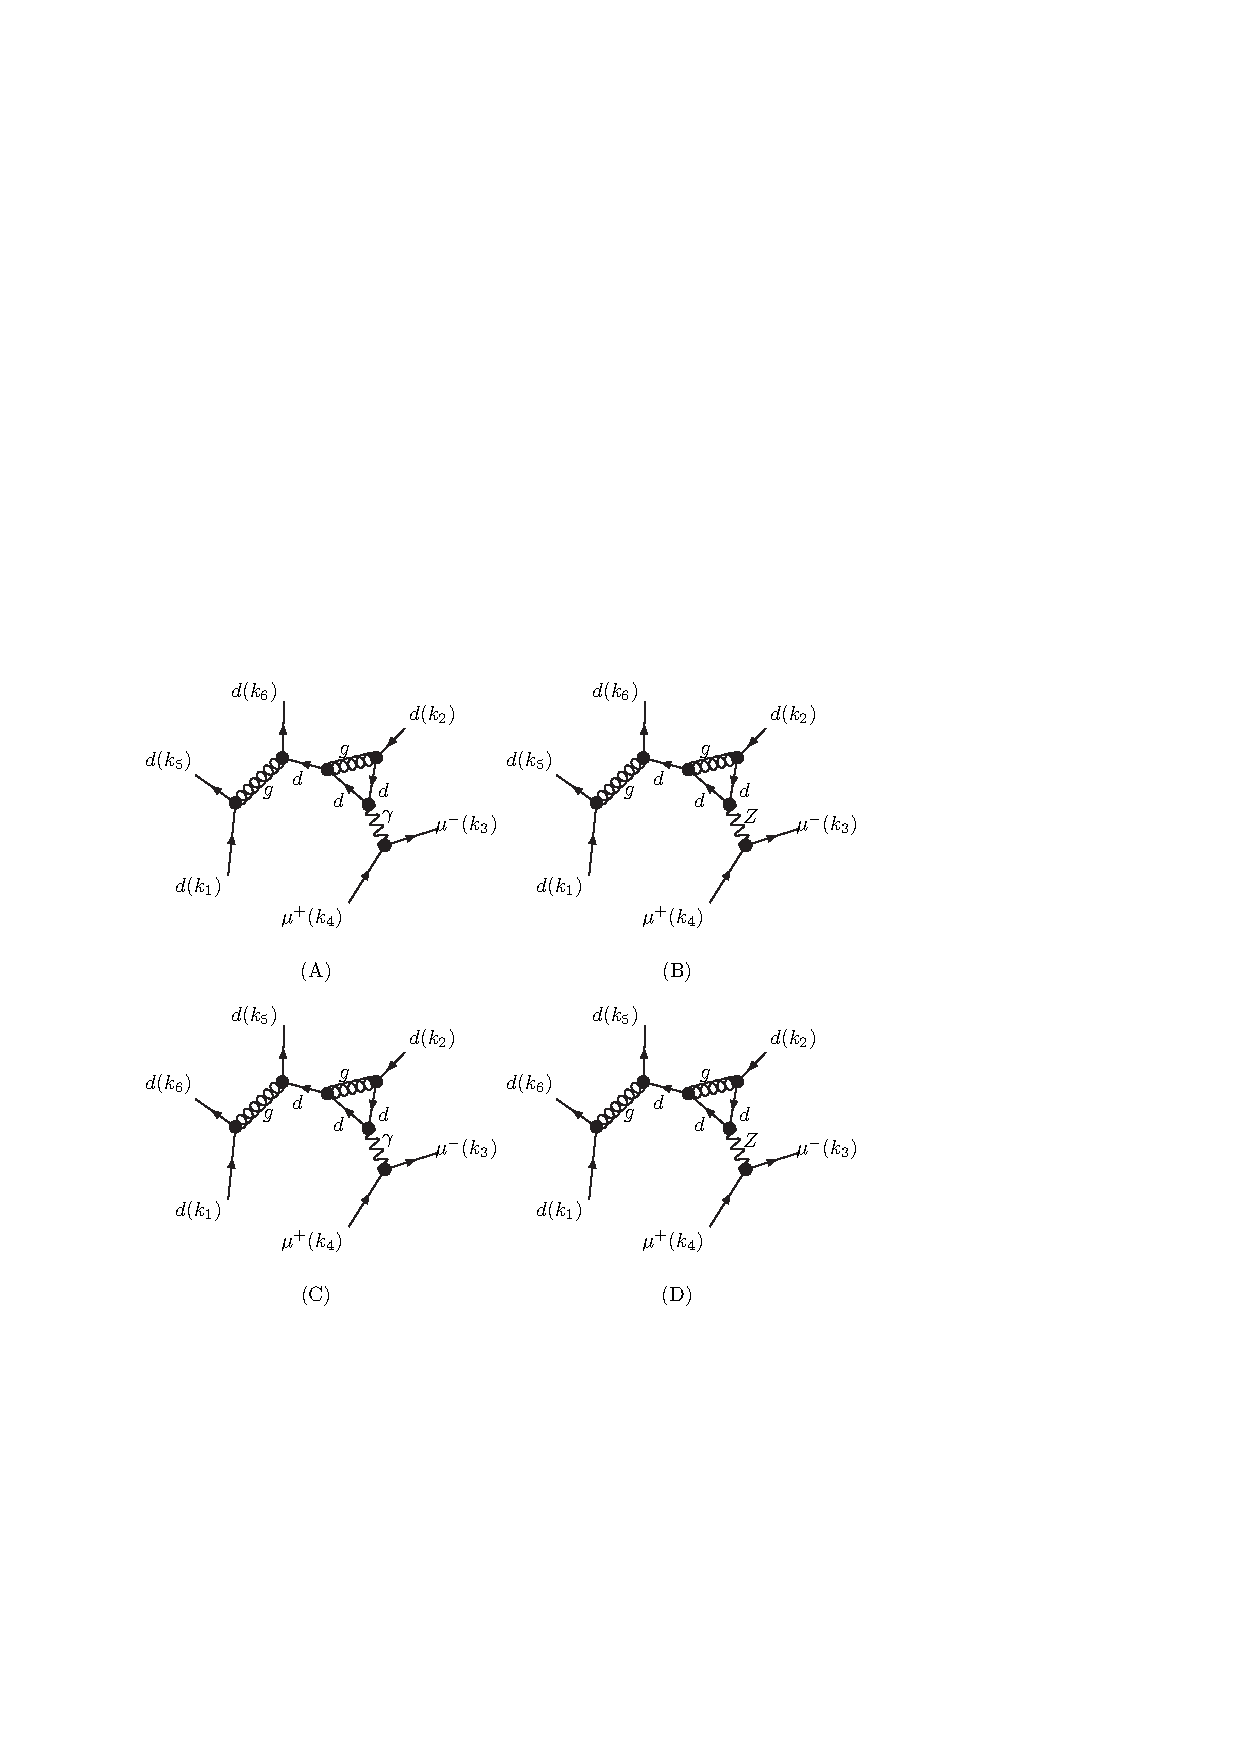
\includegraphics[width=1.0\textwidth]{diagsum1.pdf}
\caption{Example of diagrams sharing a common tree part, which are 
summed when the {\tt diagsum} option is set to {\tt diagsum=true}.}
\label{fig:diagsum_tree}
\end{figure} 

\begin{figure}[htb]
\centering
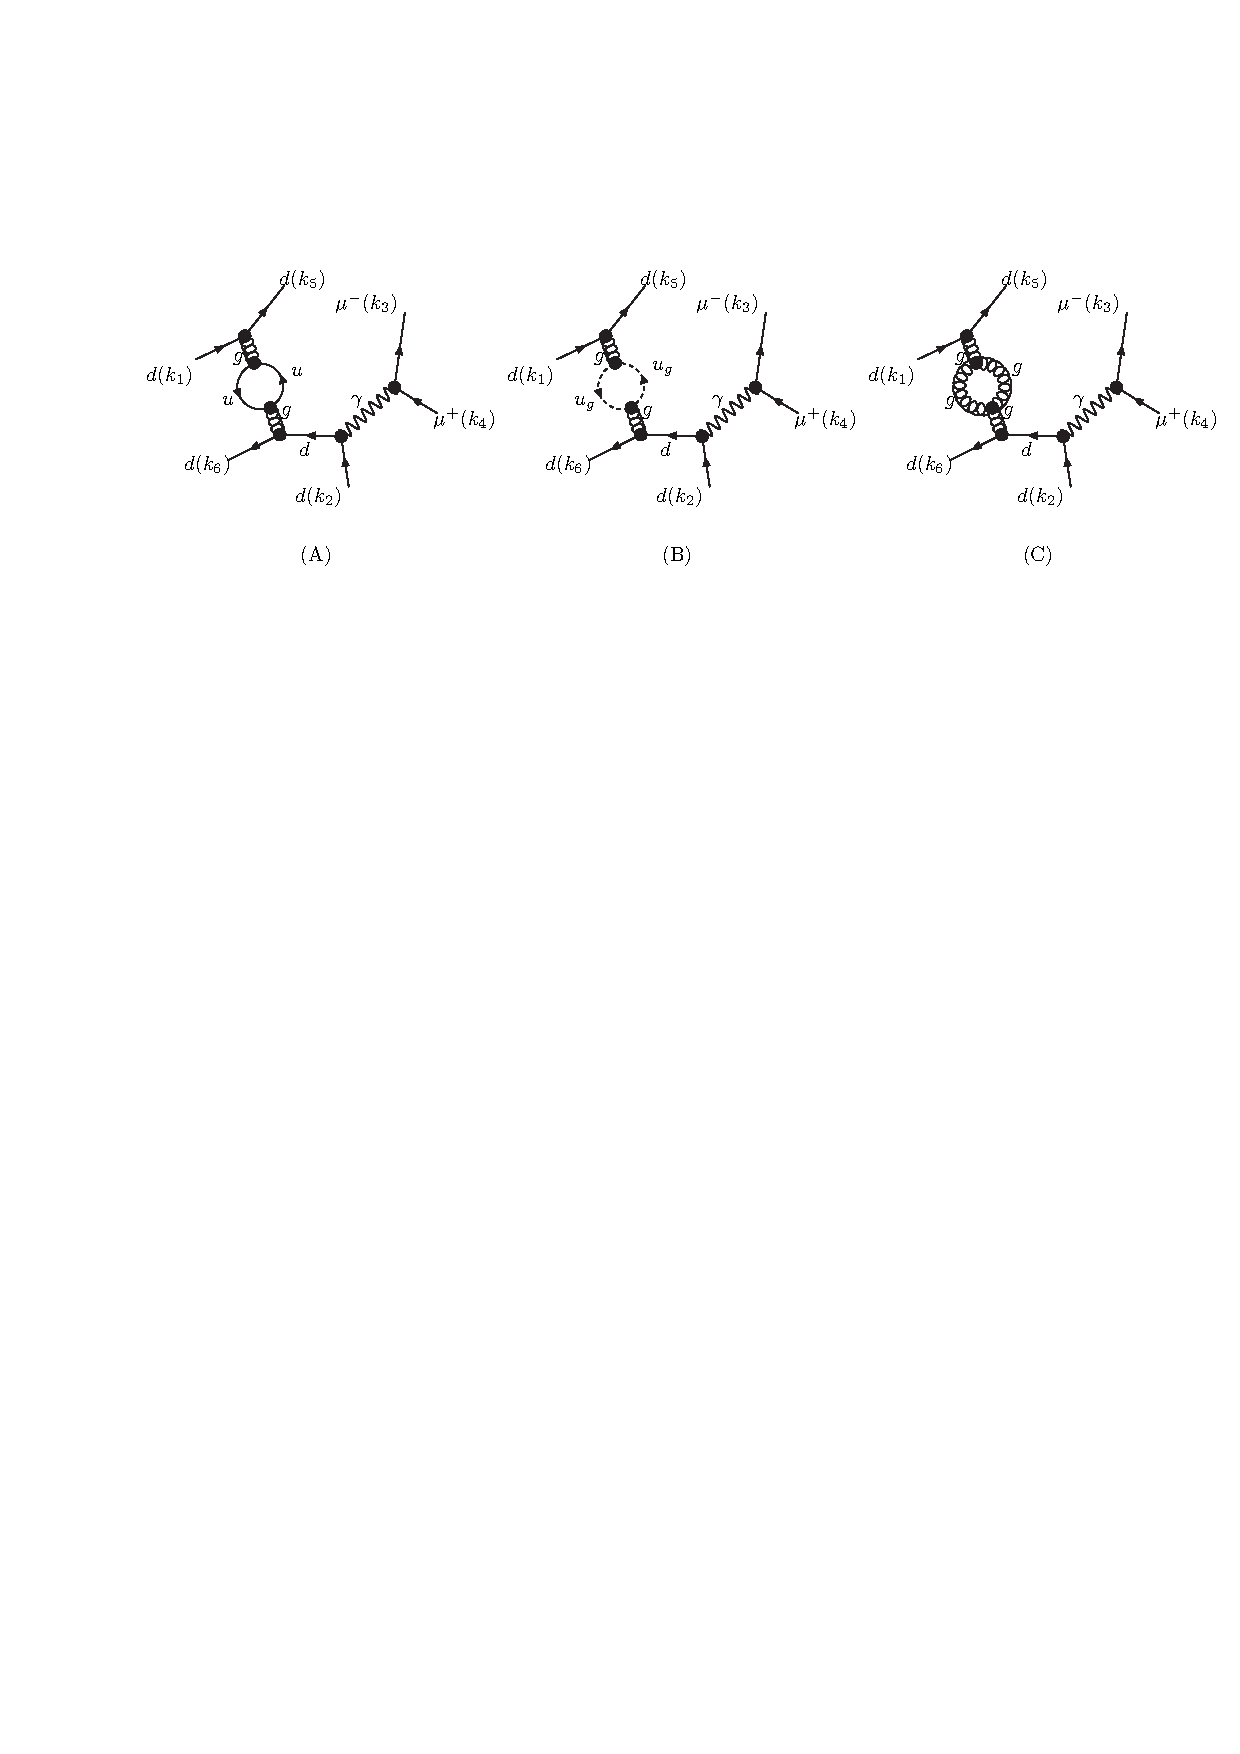
\includegraphics[width=1.1\textwidth]{diagsum2.pdf}
\caption{Example of diagrams sharing a common loop propagator, 
but with different particle content in the loop, which are summed when
the {\tt diagsum} option is set to {\tt diagsum=true}.}
\label{fig:diagsum_particle}
\end{figure} 


When the option {\tt diagsum} is active, diagrams which differ only by
a propagator external to the loop, as is the case e.g. for the
$Z/\gamma^\star$ propagator in QCD corrections to the production of
$Z+$jets, are summed together before being processed
by \form{}. Similarly, diagrams which differ only by an external tree
part, but which share exactly the same set of loop propagators, are
summed together prior the algebraic manipulation. An example is shown
Figure~\ref{fig:diagsum_tree}. Finally, diagrams which share the same
set of propagators, but have different particles circulating in the
loop, as shown in Figure~\ref{fig:diagsum_particle}, are also summed
into one ``meta-diagram''. The default setting for this option is {\tt
diagsum=true}.


\paragraph{Grouping of Tree Level Diagrams}

By default the expressions of all tree-level diagrams are grouped into one
file. This has the advantage that subexpressions which appear in several
tree-level diagrams can be reused across the amplitude. In some cases
it can happen that the sum of all terms of the tree-level diagrams is too big
to be compiled in one subroutine. In this case it is recommended to set
the option \texttt{group} to \texttt{false}. 
However, the latter can only be used in combination with the extension {\tt noformopt}.

\subsection{Numerical polarisation vectors}
\label{sec:numpolvec}
The use of numerical polarisation vectors for massless gauge bosons
(gluons, photons) is activated by default.  This means that the
various helicity configurations for the massless bosons will be
evaluated numerically, based on the same code, rather than producing
separate code for each helicity configuration.  In order to switch off
this default setting,
for example if the user would like to 
optimize the choice of reference vectors for each helicity configuration,
the option {\tt polvec=explicit} should be given in the process card 
{\tt process.in}.
In this case, \gosam{} will choose explicit reference vectors automatically.
If the user wants to specify his/her preferred reference vectors, 
this can be done using the option {\tt reference-vectors=\ldots}
in the process card.

\subsection{The extension {\tt derive}}

The {\tt derive} feature generates code to access the tensor coefficients
of each diagram or group of diagrams individually.
While it has been among the possible keywords for the 
{\tt extensions} option in \gosam-1.0 already, it now has been promoted to 
be used by default in the context of  tensorial reconstruction~\cite{Heinrich:2010ax}.
It improves both the speed and the
precision of tensorial reconstruction and makes connection to other reduction methods.

The idea behind it is to compute the numerator $\mathcal{N}(\hat{q})$ 
%--- we suppress the discussion of the second argument $\mu^2$ ---
from a Taylor series
\begin{equation}
\mathcal{N}(\hat{q})=\mathcal{N}(0)
+ \hat{q}^\mu
  \frac{\partial}{\partial\hat{q}_\mu}\mathcal{N}(\hat{q})\vert_{q=0}
+ \frac1{2!}\hat{q}^\mu\hat{q}^\nu
  \frac{\partial}{\partial\hat{q}_\mu}
  \frac{\partial}{\partial\hat{q}_\nu}
  \mathcal{N}(\hat{q})\vert_{q=0} + \ldots
\end{equation}
In this form one can read off a one-to-one correspondence between derivatives at
$\hat{q}=0$ and the coefficients of the tensor integrals.

%\paragraph{Implementation.}
At a technical level, 
the files \texttt{helicity*/d*h*l1d.f90} contain the routines
\texttt{derivative($\mu^2$, [$i_1$], [$i_2$],\dots)} and\\
\texttt{reconstruct\_d*(coeffs)}, where the latter is only generated in
conjunction with the extension \texttt{golem95}, and \texttt{coeffs} is
a type which comprises all coefficients of a diagram of a certain rank.
The number of optional indices $i_1$, $i_2$, \dots 
determine which derivative should be returned. The subroutine
\texttt{reconstruct\_d*} also takes into account the proper symmetrisation.

\subsection{Customization}
\paragraph{Runtime parameters.}
Many settings can be changed without recompiling the code, by
creating and modifying a file \texttt{matrix/param.dat}.
This file has a very simple format:
\begin{itemize}
\item Lines starting with a comment character (`!', `\#', `;')
      in the first column and blank lines are ignored.
\item All other lines have the format
\begin{example}
\textit{name} = \textit{float}\\
\# \textrm{or}\\
\textit{name} = \textit{float}, \textit{float}
\end{example}
      where the first line defines a real number and the second
      line defines a complex number, and \textit{name} is a defined
      parameter.
\item Whitespace is ignored but must not appear inside names or
      literals. Physical lines can not be continued nor can
      multiple entries appear on one line.
\end{itemize}
The list of recognized names can be found in the file
\texttt{common/model.f90}. 
With the built-in Standard Model file (\texttt{sm}) one
can re-set, for example, the value for the Higgs mass by 
{\tt mH = 125.5}.
All model constants that have not been specified as zero or one
can be set in this way. 
%Please note that upper and lower case letters have to be distinguished
%and that the names need to be spelled exactly as defined in \texttt{model.py}.
In addition there are some model independent parameters which can be found in the file 
\texttt{common/config.f90}.
%\smallskip

%\begin{tabular}{l@{\quad}p{0.7\textwidth}}
%   \texttt{samurai\_scalar} & selects a library of scalar integrals
%   (see \samurai documentation).\\
%   \texttt{samurai\_test} & sets a method to detect unstable points
%   (see \samurai documentation). \\
%   \texttt{samurai\_verbosity} & sets the verbosity level of
%   \samurai; it should be set to zero in a production environment
%   (see \samurai documentation).\\
%   \texttt{renormalisation} & An integer number indicating if no
%   renormalisation (0) or $\beta$-function renormalisation (1,
%   QCD only) should be applied. Other values are reserved for future
%   extensions. \\
%   \texttt{gauge\textit{i}o} & for the external vector particle with
%   index~$i$ (e.g. \texttt{gauge1o}, \texttt{gauge2o}\ldots),
%   if not defined as a constant. \\
%   \texttt{gauge\textit{i}z} & as \texttt{gauge\textit{i}o}.
%   The polarisation vector is transformed into
%   \begin{displaymath}
%   \varepsilon^\mu(k_i)\to\mathtt{gauge\mathit{i}o}\cdot\varepsilon^\mu(k_i)
%      + \mathtt{gauge\mathit{i}z}\cdot k_i^\mu
%   \end{displaymath}
%   This allows for a quick check of gauge invariance.
%\end{tabular}

\paragraph{Compile time parameters.}
Other configuration options can be found in the file \texttt{common/config.f90}.
%but require the recompilation of the source code
%(\texttt{make clean; make compile}).
\smallskip
Examples of options contained in \texttt{config.f90} are
\begin{maxipage}
\begin{tabular}{lp{0.6\textwidth}}
\texttt{ki} & the floating point kind used throughout the calculation, the default is double precision.\\
\texttt{debug\_lo\_diagrams} & controls if information about the
    tree level diagrams is written to the output file.\\
\texttt{debug\_nlo\_diagrams} & controls if information about the
    loop-diagrams is written to the output file.\\
\texttt{include\_eps\_terms} & controls if
    terms of order $\varepsilon$ multiplying
    poles are taken into account.\\
\texttt{include\_eps2\_terms} & controls if
    terms of order $\varepsilon^2$ multiplying
    double poles are taken into account.\\
\texttt{include\_color\_avg\_factor} & controls if the color averaging
    factor for inital state partons is multiplied to the final result.\\
\texttt{include\_helicity\_avg\_factor} & controls if the helicity averaging
    factor for inital state particles is multiplied to the final result.\\
\texttt{include\_symmetry\_factor} & controls if the symmetry
    factor for identical final state particles
    is multiplied to the final result. \\
\texttt{use\_sorted\_sum} & controls if the diagrams are summed using
    the algorithm Malcolm~\cite{Malcolm:1970}, which reduces the error
    accumulated in presence of large cancellations.\\
\texttt{tens\_rec\_by\_derivatives} & controls whether the tensorial reconstruction method is used.
\end{tabular}
\end{maxipage}

\section{Drawing the Feynman diagrams}
In order to print out the diagrams the makefile contains the target
\texttt{doc} which produces the file \texttt{process.pdf}.
We use \LaTeX{} plus the package \textsf{axodraw}~\cite{Vermaseren:1994je}
to create the graphical representation.

The layout of the diagrams is determined by the algorithm used in
\textsf{feynMF}~\cite{Ohl:1995kr}, modelling the propagators by springs.
The implemented algorithm works in two steps: first, the topology is
constructed by ordering the external legs such that the diagram can
be drawn as a planar graph. The coordinates $e_k$
of the external legs are
fixed along a contour around the drawing area.
%\footnote{Currently,
%this contour is chosen as an ellipse but in principle any convex shape could be used.}
In a second step the remaining degrees of freedom, the coordinates
of the vertices $v_i=(x_i, y_i)$, are fixed by minimizing the Lagrangian
\begin{multline}
L(v_1, \ldots, v_n; e_1, \ldots, e_N) =\\
 \frac14\sum_{i,j=1}^n t_{ij}\left(v_i-v_j\right)^2
+\frac12\sum_{i=1}^n\sum_{k=1}^N\lambda_{ik}\left(v_i-e_k\right)^2
\end{multline}
Here, $n$ is the number of vertices and $N$ is the number of external
legs.
Minimization of the Lagrangian leads to a system of linear equations, which
can easily be solved.
\begin{align*}
&\frac{\partial L}{\partial v_r}=0\\
\Leftrightarrow&
 \frac12\sum_{i,j=1}^n t_{ij}\left(v_i-v_j\right)
     \cdot\left(\delta_{ir}-\delta_{jr}\right)
+\sum_{i=1}^n\sum_{k=1}^N\lambda_{ik}\left(v_i-e_k\right)
     \cdot\delta_{ir}=0\\
\Leftrightarrow&
M_{rj}v_j\equiv
 \sum_{j=1}^n t_{rj}\left(v_r-v_j\right)
+\left(\sum_{k=1}^N\lambda_{rk}\right)v_r
=\sum_{k=1}^N\lambda_{rk}e_k
\end{align*}
In the last step we used the symmetry of $t_{ij}$.
The matrix $M$ can be written as
\begin{equation}
M_{rc}=\left\{\begin{array}{ll}
\left(\sum_{i\neq r}t_{ri}\right)+
\left(\sum_{k=1}^N\lambda_{rk}\right),&
r=c\\
-t_{rc},&\text{otherwise}
\end{array}\right.
\end{equation}

The symbol $t_{ij}$ is the sum of the spring constants of all
propagators connecting vertices $i$ and $j$; similarly, $\lambda_{ik}$
is the spring constant of the leg $k$ if it is connected to vertex $i$
and zero otherwise.

\section{Import of model files}
\label{sec:model}

The \gosam{}-2.0 package comes with the built-in model files 
{\tt sm}, {\tt smdiag}, {\tt smdiag\_mad}, {\tt smehc}, 
{\tt sm\_complex}, {\tt smdiag\_complex}, 
where the latter two are needed in the case of complex masses and couplings, 
see section \ref{sec:complexmasses}. 
The model files {\tt smdiag\_mad} contain some {\tt MadGraph5} specific settings, while
the model files {\tt smehc}  contain the effective Higgs-gluon couplings.

Other models can be imported most easily in the {\tt UFO} (Universal FeynRules Output)~\cite{Degrande:2011ua} format.
The model import in the {\tt UFO} format can be used in the standalone as well as the OLP 
mode of \gosam, where both the BLHA1 and BLHA2 standards are supported for the syntax of the model import.

Examples about how to import model files can be found in the subdirectory 
 \texttt{examples}.

\subsection{Import from FeynRules}
A model description in the UFO~\cite{Degrande:2011ua} format consists of a \texttt{Python} package
stored in a directory. In order to import the model into \gosam{} one needs
to set the \texttt{model} variable specifying the keyword \texttt{FeynRules}
in front of the directory name.
For example, if the \texttt{Python} model files for the MSSM are in 
 the directory \\
 \texttt{\$HOME/models/MSSM\_UFO}, the process card must contain the line
\begin{example}
model= FeynRules,\$HOME/models/MSSM\_UFO
\end{example}

\subsection{Import from LanHEP}
In order to use model files generated by LanHEP the following steps
have to be taken:
\begin{enumerate}
\item When generating the tables using LanHEP, one should include the
   following option to ensure that the generated tables have the correct
   headings\footnote{\gosamv{} relies on the column names rather than
   some specific order.}. The number of spaces in the column headers are
   irrelevant as long as the columns are wide enough to contain the
   respective values.
\begin{example}
   prtcformat\\
      fullname: '  fullname  ',\\
      name:     '  name   ',\\
      aname:    '  aname  ',\\
      spin2:    '  spin2  ',\\
      mass:     '  mass  ',\\
      width:    '  width  ',\\
      color:    '  color  ',\\
      aux:      '  aux  ',\\
      texname:  '      texname      ',\\
      atexname: '     atexname      ',\\
      pdg:      '  pdg   '.
\end{example}
\item If the model file is not already equipped with pdg codes
   the user might want to use the \verb!prtcprop! command in
   LanHEP to add the relevant codes.
\item In the setup file, one needs to specify the model as a pair
   of path and integer number. If the table files are under the directory
   \texttt{lanhep/ued/} in the tables \texttt{func7.mdl}, \texttt{lgrng7.mdl},
   \texttt{prtcls7.mdl} and \texttt{vars7.mdl}, the correct statement in
   the setup file would be
\begin{example}
   model=lanhep/ued, 7
\end{example}
\item The use of user defined functions (\texttt{external\_func} in LanHEP)
   requires an adaption of the file \texttt{codegen/haggies-l0.in}. If one
   wants to use the function \texttt{double foo(double,double)} the
   following line sould be added.
\begin{example}
@define mdlfoo : real, real -> real =\\ "foo(\%2\$s, \%3\$s)";
\end{example}
   The function also needs to be declared in \texttt{codegen/functions.out}
   in the subroutine \texttt{init\_functions}
\end{enumerate}


\subsection{Propagators for spin-2 particles}
\label{sec:spin2}

The propagator for massive spin-2 particles can be split into two parts
\begin{align}
	i \Delta_{\mu\nu,\rho\sigma}(k,m_{\vec n}) =  \underbrace{\frac{i}{k^2-m_{\vec n}^2 + i\epsilon}}_{D(k^2,m_{\vec n})} B_{\mu\nu,\rho\sigma}(k,m_{\vec n})\;,
\end{align}
where $B_{\mu\nu,\rho\sigma}$ carries the Lorentz structure
\begin{align}
	B_{\mu\nu,\rho\sigma}(k,m) =&
	             \left(\eta_{\mu \rho} - \frac{k_\mu k_\rho}{m^2}\right) 
		     \left(\eta_{\nu \sigma} - \frac{k_\nu k_\sigma}{m^2}\right)\notag \\
         &  + \left(\eta_{\mu \sigma} - \frac{k_\mu k_\sigma}{m^2} \right)
		     \left(\eta_{\nu \rho} - \frac{k_\nu k_\rho}{m^2}\right) \notag \\
         &  - \frac23  
	   \left(\eta_{\mu \nu} - \frac{k_\mu k_\nu}{m^2}\right)
	   \left(\eta_{\rho \sigma} - \frac{k_\rho k_\sigma}{m^2}\right)\;.
\end{align}
%and 
%\be
%D(s,m_{\vec n}) =  \frac{i}{s-m_{\vec n}^2 + i \epsilon}\;.
%\ee
If all particles attached to the propagator are on-shell, 
the mass dependent terms in $B_{\mu\nu,\rho\sigma}(k,m)$ drop out.
Further, if the on-shell condition is not always fulfilled, 
it turned out in phenomenological applications that the impact of the mass dependent terms is numerically 
negligible\,\cite{Gleisberg:2003ue,Greiner:2013gca}
and therefore we did not include them in our implementation
in order to avoid an enormous proliferation of terms.
In this case the summation over the graviton states  in $D(s,m_{\vec n})$, leading to
\be
D(s) = \sum_{\vec n} \frac{i}{s-m_{\vec n}^2 + i \epsilon}\;,
\ee
can be performed independently from the  $B_{\mu\nu,\rho\sigma}$ part carrying the Lorentz structure.
Further, in  models with large extra dimensions (LED),
 we can use the assumption that the widths of the KK modes are negligible, 
as the dominant effects come from the almost on-shell production of KK modes, 
and that the discrete spectrum of the KK  modes can be approximated by an
integral over a mass density, as the  KK modes are very contiguous.
%\,\cite{Han:1998sg,Giudice:1998ck}. 
The density as a function of the mass $m_{\vec n}$ is given by
\be
\rho(m_{\vec n})=\frac{R^{\delta}m_{\vec n}^{\delta - 2}}{(4\pi)^{\delta/2}\Gamma(\delta/2)}\;,
\ee
where $\delta$ is the number of extra dimensions, leading to \,\cite{Han:1998sg}
\begin{align}
	D(s) \to  \int_0^{M_S} d\,m_{\vec n}^2\,
	\frac{i\,\rho(m_{\vec n})}{s-m_{\vec n}^2+ i \epsilon}
	= \begin{cases} \frac{ s^{\delta/2-1}}{2M_{s}^{\delta + 2} G_N } \left( \pi + 2 i \, I(\frac{M_S}{\sqrt{s}}) \right) & \text{for\ } s>0 \\
		\frac{ (-s)^{\delta/2-1}}{2M_{s}^{\delta + 2} G_N} (-2i)\, I_E(\frac{M_S}{\sqrt{-s}}) & \text{for\ } s<0 
	\end{cases}
	\label{eq:propagator}
\end{align}
with 
\begin{align}
	I(x) = \begin{cases} - \sum_{k=1}^{\delta/2-1} \frac1{2k} x^{2k} - \frac12 \log(x^2-1)& \text{if\ } \delta \text{ even} \\
		- \sum_{k=1}^{(\delta-1)/2 } \frac{1}{2k-1} x^{2k-1} + \frac12 \log\left( \frac{x+1}{x-1} \right) & \text{if\ } \delta \text{ odd}
	\end{cases}
\end{align}
and
\begin{align}
	I_E(x) = \begin{cases} (-1)^{\delta/2 + 1} \left( \sum_{k=1}^{\delta/2-1} \frac{(-1)^k}{2k} x^{2k} + \frac12 \log(x^2+1)  \right) 
		& \text{if } \delta \text{ even} \\
		(-1)^{(\delta-1)/2} \left(   \sum_{k=1}^{(\delta-1)/2 } \frac{(-1)^k}{2k-1} x^{2k-1} + \frac12 \tan^{-1}(x) \right)   & \text{if } \delta \text{ odd} \,.
	\end{cases}
\end{align}
The UV cutoff $M_S$ is introduced as the effective theory approach loses its validity beyond the scale $M_S$.


\gosam{} supports spin-2 propagators with the \texttt{customspin2propagator} extension which
needs to be enabled in the process card by \\
{\tt extensions=customspin2propagator}.

The extension works only if the model is imported from an {\tt UFO} file. 
The latter can  be adjusted to the needs of the particular model the 
user would like to consider by editing the file {\tt custompropagator.f90}
in the subdirectory {\tt common}. 
In order to generate the latter file,
the spin-2 particle which should get a customized propagator needs to have a
separate attribute 'CustomSpin2Prop' in the {\tt UFO} file with a non-vanishing
value:\\
Excerpt of {\tt LED\_UFO/particle.py} with a customized propagator:
\begin{verbatim}
    Gr = Particle(pdg_code = 9000006,
                  name = 'Gr',
                  # ...
                  CustomSpin2Prop = 1
                 )
\end{verbatim}
Then \gosam{} generates a the file {\tt common/custompropagator.f90} where the user needs
to adapt the {\tt customSpin2Prop} subroutine.
Beside the squared momentum, the {\tt customSpin2Prop} subroutine also receives the
mass of the corresponding spin-2 particle as an argument, which
can be used to distinguish between multiple spin-2 particles if necessary.
The tensorial part of the spin-2 propagator, $B_{\mu\nu,\rho\sigma}(k,m_{\vec n})$, is treated separately 
and should not be modified.  If the user would like to modify it, we refer to the  documentation in 
section 6.3 of {\tt src/form/lorentz.pdf} in the \gosam{} tarball.



%\section{Handling big processes}
%Although the default settings should work for most cases, very big processes
%in terms of the number of diagrams and the size of the expressions can cause
%the compiler to become very slow or even to crash. In this section we discuss
%solutions which can help to reduce the load for the compiler and to speed-up
%the code generation. It should be mentioned that some of these measures can
%have a negative impact on the runtime efficiency of the generated code.



%%%%%%%%%%%%%%%%%%%%%%%%%%%%%%%%%%%%%%%%%%%%%%%%%%%%%%%%%%%%%%%%%%%%%%%%%%%

\chapter{Stability tests and rescue system}
\label{sec:rescue}

\gosam{} contains various options to assess in real time, for each phase space point, 
the level of precision of the corresponding one-loop matrix element. 
Whenever a phase space point is found in which the quality of the result falls below a
certain threshold, either the point is discarded or the evaluation of the amplitude is
repeated by means of a safer, albeit less efficient procedure. This procedure is
traditionally called ``rescue system''.

Apart from improvements in the stability of the reduction itself, which are provided by the new versions of \samurai{} and \golemVC, and in particular by the new reduction algorithm \ninja,  the new version of \gosam{} also has a more refined rescue system as compared to version 1.0. 

A first commonly used approach relies on the comparison between the numerical values of the
infrared pole coefficients computed by the one-loop program with 
their known analytic results dictated by the universal behaviour of the 
infrared singularities~\cite{Catani:2000ef}. We refer to this as the {\it pole test}. 

The main advantages of this method are its broad applicability and the fact that it requires a negligible additional computation time. However, since not all integrals which appear in the reconstruction of the amplitude give a contribution to the double and single poles, this method often provides an overestimate of the precision, which might result in keeping  phase space points whose finite part is less precise than what is predicted by the pole test.

To target directly the precision of the finite part, various possibilities exist.
Using the symmetry properties of scattering amplitudes under scaling of all physical scales,
 or alternatively the invariance under rotation of the momenta, 
 we can build pairs of points that should provide identical results, 
 both for the finite parts and for the poles, and use the difference between them 
 as an estimator of the precision. 

The {\it scaling test}~\cite{Badger:2010nx}, is based on the properties of scaling of scattering amplitudes when all physical scales (momenta, renormalization scale, masses) are rescaled by a common multiplicative factor $x$. As shown in~\cite{Badger:2010nx}, this method provides a very good correlation between the estimated precision and the actual precision of the finite parts.

The {\it rotation test}~\cite{vanDeurzen:2013saa} exploits the invariance of the scattering amplitudes under an azimuthal rotation about the beam axis, namely the direction of the initial colliding particles. Whenever the initial particles are not directed along the beam axis, one can perform a rotation of all particles by an arbitrary angle in the space of momenta. A validation of this technique, and the corresponding correlation plots, has been presented in~\cite{vanDeurzen:2013saa}.

While  the {\it scaling} and the {\it rotation test} provide a more reliable estimate of the precision of the finite parts that enter in the phase space integration, their downside is that they require two evaluations of the same matrix element, therefore leading to a doubling in the computational time.

%Additional methods have been proposed, within the context of integrand-reduction approaches, which target the relations between the coefficients before integration, namely the reconstructed algebraic expressions for the numerator function before integration, known as  $\N=\N$ tests~\cite{Ossola:2007ax, Mastrolia:2010nb}.
%This kind of tests can be applied to the full amplitude (global   $\N=\N$ test) or individually within each residue of individual cuts (local $\N=\N$ test). The drawback of this technique comes from the fact that the test is applied at the level of individual diagrams, rather than on the final result summed over all diagrams, making the construction of a rescue system quite cumbersome. 

For the precision analysis contained in \gosamv, and to set the trigger for the rescue system, we decided to employ  a hybrid method, that takes advantage of the computational speed of the {\it pole test}, combined with the higher reliability of the {\it rotation test}.  This hybrid method requires setting three different thresholds.
After computing the matrix elements, \gosamv{} checks the precision  $ \delta_{pole}$ of the single pole with the {\it pole test}. Comparing the single pole 
$\S_{IR}$ that can be obtained from the general structure of infrared singularities and the one provided by  \gosamv, which we label $\S$, we define  
\be \label{eq:exd}
\delta_{pole} = \left | \frac{ \S_{IR} - \S{} }{ \S_{IR}} \right |\, .
\ee
The corresponding estimate of the number of correct digits in the result is provided by  $P_{pole}= - \log_{10} (\delta_{pole})$. This step does not require any increase in computational time. The value of $ P_{pole}$ is then compared with two thresholds $ P_{high}$ and $ P_{low}$. 

If $P_{pole} >  P_{high}$ the point is automatically accepted. Given the high quality of the computed pole, the finite part is very unlikely to be so poor that the point should be discarded.

If $P_{pole} <  P_{low}$ the point is automatically discarded, or sent to the rescue system. If already the pole has a low precision, we can expect the finite part to be of the same level or worse.
 
In the intermediate region where $ P_{high} > P_{pole} >  P_{low}$, it is more difficult to determine the quality of the result solely based on the pole coefficients. Only in this case the point is recalculated using the {\it rotation test}, which requires additional computational time. 

If we call the finite part of the amplitudes evaluated before and after the rotation $\A$ and  $\A_{rot}$ respectively,  we can define the error $ \delta_{rot}$ estimated with the rotation  as  
\be  \label{eq:errd} \delta_{rot} =  2 \left  |\frac{ A_{rot} - A }{ A_{rot} + A} \right  |\, . \ee
and the corresponding estimate on the number of correct digits as $P_{rot} = - \log_{10} (\delta_{rot})$.
$P_{rot}$ provides a reliable estimate of the precision of the finite part~\cite{vanDeurzen:2013saa}, and can be compared with a threshold $P_{set}$ to decide whether the point should be accepted or discarded. 

The values of the three thresholds $ P_{high} $,  $P_{low}$ and $P_{set}$ can be chosen by the user, to adjust the selection mechanism to the fluctuations in precision which occur between different processes. In the input card, $ P_{high} $,  $P_{low}$ and $P_{set}$ correspond to 
\texttt{PSP\_chk\_th1}, \texttt{PSP\_chk\_th2} and \texttt{PSP\_chk\_th3}, 
respectively, see section \ref{chp:setup-of-a-process}.
It is worth to notice that the {\it rotation test} can be bypassed simply by setting the initial thresholds $P_{high}= P_{low}$. In this case the selection is performed solely on the basis of the {\it pole test}.


%%%%%%%%%%%%%%%%%%%%%%%%%%%%%%%%%%%%%%%%%%%%%%%%%%%%%%%%%%%%%%%%%%%%%%%%%%%
\chapter{Electroweak corrections}


\section{Electroweak scheme choice}
\label{sec:ewchoose}
When computing amplitudes within the Standard Model, there are different
possibilities how to choose which electroweak parameters are
considered as input parameters, and which are instead derived
ones. Within \gosam{} different schemes can be chosen in several
different ways, depending on whether the scheme might be changed after
the generation of the code or not, by setting appropriately the flag
{\tt model.options}.

By default, when the flag is not set in the input card, \gosam{}
generates a code which uses $\mrm{m_W}$, $\mrm{m_Z}$ and
$\mrm{\alpha}$ as input parameters, allowing however to change this in
the generated code, by setting the variable {\tt ewchoice} in the
configuration file {\tt config.f90} to the desired value. The user can
choose among 8 different possibilities, which are listed in
Table~\ref{tab:ewchoose}.  When the electric charge $\mrm{e}$ is set
algebraically to one, the schemes $6-8$ cannot be used.

\begin{table*}
\begin{center}
\small
\begin{tabular}{|c|l|l|}
\hline
ewchoice & input parameters                        & derived parameters                  \\
\hline
1        & $\mrm{G_F}$, $\mrm{m_W}$, $\mrm{m_Z}$    & $\mrm{e}$, $\mrm{sw}$              \\
2        & $\mrm{\alpha}$, $\mrm{m_W}$, $\mrm{m_Z}$ & $\mrm{e}$, $\mrm{sw}$              \\
3        & $\mrm{\alpha}$, $\mrm{sw}$, $\mrm{m_Z}$  & $\mrm{e}$, $\mrm{m_W}$             \\
4        & $\mrm{\alpha}$, $\mrm{sw}$, $\mrm{G_F}$  & $\mrm{e}$, $\mrm{m_W}$             \\
5        & $\mrm{\alpha}$, $\mrm{G_F}$, $\mrm{m_Z}$ & $\mrm{e}$, $\mrm{m_W}$, $\mrm{sw}$ \\
6        & $\mrm{e}$, $\mrm{m_W}$, $\mrm{m_Z}$      & $\mrm{sw}$                         \\
7        & $\mrm{e}$, $\mrm{sw}$, $\mrm{m_Z}$       & $\mrm{m_W}$                        \\
8        & $\mrm{e}$, $\mrm{sw}$, $\mrm{G_F}$       & $\mrm{m_W}$, $\mrm{m_Z}$           \\
\hline
\end{tabular}
\end{center}
\caption{Possible choices to select the electroweak scheme.
To simplify the notation we write the sine of the Weinberg angle as
$\mrm{sw}$. The lists of derived parameters contain only the
parameters which are computed and used in the expressions for the
amplitudes.}\label{tab:ewchoose}
\end{table*}


The flag {\tt model.options} in the input card allows also to directly
set the values of the different parameters appearing in the model. If
the values of exactly three electroweak parameters are
specified, \gosam{} automatically takes them as input parameters. In
that case, in order to be able to switch among different schemes after
code generation, the variable {\tt ewchoose} also must be added to the
{\tt model.options} flag.



\section{Support of complex masses}
\label{sec:complexmasses}
The integral libraries contained in the \gosam{} package as well as the \gosam{} 
code itself fully support complex masses. This refers to the introduction of 
finite widths for fermions as well as
for $W$- and $Z$-bosons. A fully consistent treatment of complex
$W$- and $Z$-boson masses requires the use of the complex mass scheme~\cite{Denner:2005fg}.
The boson masses are promoted to complex masses by
\begin{equation}
 m_{V}^2 \to \mu_{V}^2 = m_{V}^2 -i m_{V} \Gamma_{V},\quad V=W,Z\;.
\end{equation}
In order to maintain gauge invariance this affects the definition of the Weinberg angle:
\begin{equation}
 \cos^2\theta_w = \frac{\mu_W^2}{\mu_Z^2}\;.
\end{equation}
 To make use of the complex mass scheme, we introduce two new model files, \texttt{sm\_complex}
 and \texttt{smdiag\_complex}, which contain the Standard Model with complex mass scheme, the first
 with a full CKM matrix, the latter with a diagonal  CKM matrix.
 An example dealing with a complex top quark mass is given in 
 the {\tt examples/singletop} subdirectory of the \gosam{} distribution.

%\subsection{Splitting the Process}
%If a process becomes too big in order to be linked\footnote{
%Currently, most systems support programs to a size up to 4\,GB.
%Although 64\,bit systems can handle a much bigger address space,
%the current limitation comes from some legacy code in the GNU linker.}
%there are some possibilities to split the process into independent
%programs:
%\begin{itemize}
%\item the generation of a subset of the helicity configurations, 
%e.g. one helicity configuration      per process directory.
%\item the generation of a subset of diagrams. If the diagrams are not
%      split according to gauge invariant subsets the user should ensure
%      that all subsets are called with the same set of phase space points.
%      An easy way of splitting the diagrams into subsets is by using
%      the option \texttt{select.nlo=\textit{$\langle$first$\rangle$}:\textit{%
%       $\langle$last$\rangle$}}, where \texttt{first} and \texttt{last} refer to the 
%       diagram numbers in {\em process.ps}.
%\end{itemize}

%\section{Advanced Usage}
%The call to the executable \texttt{gosam.py} can be simulated
%inside more complex \python programs.
%It is an easy exercise to
%run the file generation in user defined \python scripts as long as
%one includes the module files in the environment variable
%\texttt{PYTHON\_PATH}. The following script emulates the
%program \texttt{gosam.py}:
%\begin{lstlisting}[language=python]
%>>> from golem.util.config import Properties
%>>> from golem.util.main_misc import *
%>>> props = Properties()
%>>> props.setProperty("in", ["e+", "e-"])
%>>> props.setProperty("out", ["t", "t~"])
%>>> # ... populate props with further values ...
%>>> workflow(props)
%>>> generate_process_files(props)
%\end{lstlisting}

\chapter{Advanced diagram selection}
\gosamv implements several ways of selecting subsets of diagrams:
\begin{itemize}
\item by restricting QGraf,
\item by selecting specific diagrams by their number,
\item by defining filters using \python.
\end{itemize}

\section{Restricting the generation with QGraf}
The options for restricting the set of diagrams at the level
of the diagram generation is the most efficient way since this
happens already at the earliest possible stage.
However, QGraf's built-in filters are sometimes
too limited in order to express more advanced criteria.

\gosamv{} allows one to pass information to QGraf through the option
\texttt{qgraf.options} and through \texttt{qgraf.verbatim},
\texttt{qgraf.verbatim.lo} and \texttt{qgraf.verbatim.nlo}.
For the exact syntax the user is referred to the examples and 
to the QGraf documentation.

\section{Selecting diagrams by their number}
An a posteriori selection 'by eye' can be achieved after all (also unwanted)
diagrams of a process have been generated and inspected in
\texttt{doc/process.ps}. The user can then modify the options
\texttt{select.lo} and \texttt{select.nlo} and rerun \texttt{gosam.py}.

%This option is mainly intended for debugging purposes in large processes.

\section{Filtering diagrams in \python{}}
\label{sec:filter}
The user can write short \python{} functions in order to decide whether
a specific diagram is to be taken or not. This function should return
\texttt{True} for all diagrams which are kept, and \texttt{False} for
all diagrams which should be discarded. These functions are passed by
the options \texttt{filter.lo} and \texttt{filter.nlo}.

Longer functions should be defined in an external file, which can be
passed using \texttt{filter.module}.

When writing a filter the one can use the predefined particle lists
\texttt{QUARKS}, \texttt{LEPTONS}, \texttt{FERMIONS} and \texttt{BOSONS}.
The underscore (\texttt{\_}) matches any field.

A diagram object \texttt{d} has the following methods which are inteded
to be used in filters.
Alternative predefined functions and functors are also given.
\begin{description}
\item[\texttt{d.rank()}] returns the tensor rank of a diagram.\\
   $\mathtt{RANK}\equiv\lambda\mathtt{d}.(\mathtt{d.rank()})$
\item[\texttt{d.loopsize()}] returns the number of propagators
   in the loop of a diagram.\\
   $\mathtt{LOOPSIZE}\equiv\lambda\mathtt{d}.(\mathtt{d.loopsize()})$
\item[\texttt{d.sign()}] computes the sign coming from closed
   fermion loops.\\
   $\mathtt{SIGN}\equiv\lambda\mathtt{d}.(\mathtt{d.sign()})$
\item[\texttt{d.isNf()}] reports if a diagram contains a closed
   quark loop of size two where all loop propagators are massless.\\
   $\mathtt{NF}\equiv\lambda\mathtt{d}.(\mathtt{d.isNf()})$
\item[\texttt{d.isMassiveQuarkSE()}] returns True if the diagram
   contains a QCD self energy insertion at a massive quark line.\\
   $\mathtt{MQSE}\equiv\lambda\mathtt{d}.(\mathtt{d.isMassiveQuarkSE()})$
\item[\texttt{d.isScaleless()}] returns True if the loop integral associate
   with this diagram carries no scale.\\
   $\mathtt{SCALELESS}\equiv\lambda\mathtt{d}.(\mathtt{d.isScaleless()})$
\item[\texttt{d.vertices(f1,f2,\ldots)}] returns the number of vertices
   in the diagram with the specified fields. The arguments \texttt{f1},
   \texttt{f2}, \dots are lists of field names.\\
   $\mathtt{VERTICES(f1,f2,\ldots)}\equiv
    \lambda\mathtt{d}.(\mathtt{d.vertices(\mathtt{f1},\mathtt{f2},\ldots)})$
\item[\texttt{d.loopvertices(f1,f2,\ldots)}]
   same as \texttt{vertices}, but only counts vertices which have
   loop propagators attached.\\
   $\mathtt{LOOPVERTICES(f1,f2,\ldots)}\equiv
    \lambda\mathtt{d}.(\mathtt{d.loopvertices(
    \mathtt{f1},\mathtt{f2},\ldots)})$
\item[\texttt{d.iprop(f,**opts)}] returns the number of propagators
   of the given fields. Optional arguments are
   \texttt{momentum} to specify the momentum of the propagator,
   \texttt{twospin} to filter by the $2\times$ the spin,
   \texttt{massive} to specify whether massive or massless propagators
   should be considered and \texttt{color} to filter for certain color
   representations.\\
   $\mathtt{IPROP(\ldots)}\equiv
    \lambda\mathtt{d}.(\mathtt{d.iprop(\ldots)})$
\item[\texttt{d.chord(f,**opts)}] same as \texttt{iprop}
   but only counts loop propagators.\\
   $\mathtt{CHORD(\ldots)}\equiv
    \lambda\mathtt{d}.(\mathtt{d.chord(\ldots)})$
\item[\texttt{d.bridge(f,**opts)}] same as \texttt{iprop}
   but only counts propagators which are not in a loop.\\
   $\mathtt{BRIDGE(\ldots)}\equiv
    \lambda\mathtt{d}.(\mathtt{d.bridge(\ldots)})$
\item[\texttt{d.QuarkBubbleMasses()}] returns a list of
   all different masses in a closed quark loop of size two
   or an empty list if the diagram is not a quark bubble.\\
   $\mathtt{QBMASSES}\equiv
    \lambda\mathtt{d}.(\mathtt{d.QuarkBubbleMasses()})$
\end{description}

Furthermore, the following predefined filters exist:
\begin{description}
\item[\texttt{NFGEN(f1,f2,\ldots)}] for closed quark loops of size two
   this filter returns true only if all loop propagators belong to one
   of the fields in the argument list. For all diagrams which are not
   quark bubbles it returns True.
\item[\texttt{AND(filter1,filter2,\ldots)}] returns True if all filters
   in the argument list return True.
\item[\texttt{OR(filter1,filter2,\ldots)}] returns True if at least one filter
   in the argument list returns True.
\item[\texttt{NOT(filter)}] returns True if the argument evaluates to False.
\item[\texttt{TRUE}] always returns True.
\item[\texttt{FALSE}] always returns False.
\end{description}

%%%%%%%%%%%%%%%%%%%%%%%%%%%%%%%%%%%%%%%%%%%%%%%%%%%%%%%%%%%%%%%%%%
%% BLHA.tex is a separate file, was used for the version 1.0 manual
%\documentclass[a4paper]{refart}
%\usepackage{listings}
%\usepackage{color}
%\usepackage{amsmath}
%\title{GoSam BLHA Interface How-To}
%\author{T. Reiter, G.~Luisoni}
%\definecolor{lstbg}{rgb}{0.9,0.9,0.9}
%\lstset{basicstyle=\tt,backgroundcolor=\color{lstbg}}
%\begin{document}
%\maketitle
%\tableofcontents

\chapter{The Binoth Les Houches Accord Interface}
\label{sec:blha}


The interface of \gosam{} with a Monte Carlo event generator program 
is based on the Binoth-Les Houches Accord (BLHA)
standard interface.
\gosam{}-2.0 supports both BLHA1~\cite{Binoth:2010xt}
and BLHA2~\cite{Alioli:2013nda}.
Certainly, a dedicated interface without using the BLHA is also possible.

%We assume that \gosam{} has been downloaded and installed using the script
%\texttt{gosam-installer.py} which comes with the distribution. 
%You should ensure
%that the file \texttt{gosam.py} is in your \texttt{\$PATH} variable.


\section{Preparation of the order file}
This step should be done by the Monte Carlo (MC) program. 
We give a generic example of an order file for the process \\
$pp\to (Z\to e^+e^-)+$\,jet in both BLHA1 and BLHA2 standards 
in Figs.~\ref{fig:BLHA1} and \ref{fig:BLHA2}.
%in the files \texttt{order1.lh} \texttt{order2.lh}  
\begin{figure}[htb!]
\begin{subfigure}[]{0.49\textwidth}
%\framebox(158,210){%
\fbox{
    \parbox[t][][c]{145\unitlength}{\tt\scriptsize
\# OLP\_order.lh   \\
\# created by MC Sherpowig-1.0\\
\# Process: p p $->$ e+ e- jet\\
Model                    SMdiag\\
CorrectionType           QCD\\
IRregularisation         DRED\\
AlphasPower              2\\
AlphaPower               1\\
MatrixElementSquareType  CHsummed\\
OperationMode            CouplingsStrippedOff\\
SubdivideSubprocess      no\\
\# Subprocesses \\
1 -1 $->$ 11 -11 21\\ 
1 21 $->$ 11 -11 1\\
2 -2 $->$ 11 -11 21\\
...\\
21 -2 $->$ 11 -11 -2\\
\\
\# Process specific GoSam settings\\
\#@ symmetries family,generation}
}
\end{subfigure}
\begin{subfigure}[]{0.49\textwidth}
%\framebox(178,210){%
\fbox{
    \parbox[t]{165\unitlength}{\tt\scriptsize
\# vim: syntax=olp\\
\#@OLP GOSAM 2.0\\
\#@IgnoreUnknown False\\
\#@IgnoreCase False\\
\#@SyntaxExtensions \\
CorrectionType QCD $|$ OK\\
IRregularisation DRED $|$ OK\\
AlphasPower 2 $|$ OK\\
AlphaPower  1   $|$ OK\\           1\\
MatrixElementSquareType CHsummed $|$ OK\\
OperationMode CouplingsStrippedOff $|$ OK\\
SubdivideSubprocess  no $|$ OK\\
1 -1 $->$ 11 -11 21 $|$ 1 1\\
1 21 $->$ 11 -11 1  $|$ 1 2\\
2 -2 $->$ 11 -11 21 $|$ 1 3\\
...\\
21 -2 $->$ 11 -11 -2 $|$ 1 13\\}
}
\end{subfigure}
\caption{Examples of order and contract files for Z+jet, with BLHA1 standards.}
\label{fig:BLHA1}
\end{figure}  



\begin{figure}[h]
\begin{subfigure}[]{0.49\textwidth}
%\framebox(150,310){%
\fbox{
    \parbox[t][][b]{148\unitlength}{\tt\scriptsize
\#  OLP\_order.lh \\
\# created by MC Sherpowig-2.0\\
InterfaceVersion         BLHA2\\
CorrectionType           QCD\\
IRregularisation         DRED\\
WidthScheme              ComplexMass\\
EWScheme                 alphaGF\\
AccuracyTarget           0.0001\\
DebugUnstable            True\\

AlphasPower              1\\
AmplitudeType ccTree\\
1 -1 $->$ 11 -11 21 \\
...\\
21 -2 $->$ 11 -11 -2 \\
AmplitudeType scTree\\
1 -1 $->$ 11 -11 21 \\
...\\
21 -2 $->$ 11 -11 -2 \\
AmplitudeType Loop\\
1 -1 $->$ 11 -11 21 \\
...\\
21 -2 $->$ 11 -11 -2 \\
\\
AlphasPower              2\\
AmplitudeType Tree\\
1 1 $->$ 11 -11 1 1 \\ 
...\\
21 21 $->$ 11 -11 2 -2\\}}
\end{subfigure}
%\parbox{5\unitlength}{}
\begin{subfigure}[]{0.49\textwidth}
%\framebox(163,310){%
\fbox{
    \parbox[t][][b]{160\unitlength}{\tt\scriptsize
\# vim: syntax=olp\\
\#@OLP GOSAM 2.0\\
\#@IgnoreUnknown False\\
\#@IgnoreCase False\\
\#@SyntaxExtensions \\
InterfaceVersion BLHA2 $|$ OK\\
CorrectionType QCD $|$ OK\\
IRregularisation DRED $|$ OK\\
WidthScheme              ComplexMass $|$ OK\\
EWScheme                 alphaGF $|$ OK\\
AccuracyTarget           0.0001 $|$ OK\\
DebugUnstable            True $|$ OK\\

AlphasPower 1 $|$ OK\\
AmplitudeType ccTree $|$ OK\\
1 -1 $->$ 11 -11 21 $|$ 1 131\\
...\\
21 2 $->$ 11 -11 2 $|$ 1 70\\
AmplitudeType scTree | OK\\
1 -1 $->$ 11 -11 21 $|$ 1 145\\
...\\
21 2 $->$ 11 -11 2 $|$ 1 71\\
AmplitudeType Loop $|$ OK\\
1 -1 $->$ 11 -11 21 $|$ 1 137\\
...\\
21 2 $->$ 11 -11 2 $|$ 1 63\\
\\
AlphasPower 2 $|$ OK\\
AmplitudeType Tree $|$ OK\\
1 1 $->$ 11 -11 1 1 $|$ 1 42\\
...\\
21 21 $->$ 11 -11 -2 2 $|$ 1 106\\}
}
\end{subfigure}
\caption{Order and contract files for Z+jet with BLHA2 standards.}
\label{fig:BLHA2}
\end{figure}  

\paragraph{Remarks}
\begin{itemize}
\item The order file can have any name and any extension.
      We use  the extension \texttt{.lh}
      for order files and \texttt{.olc} for contract files.
\item The options \texttt{WidthScheme, EWScheme} in the BLHA2  example are optional.
\item The option \texttt{SubdivdeSubprocess}  has the following effect
      on the code generation with \gosam{}: if set to 
      \texttt{no}, \gosam{} generates one label per subprocess, if set to
      \texttt{yes} it generates one label per helicity subamplitude
      and therefore \emph{many} labels per subprocess.
      
\item \gosam{} specific settings can be put into commentary lines starting
      with the letter combination `\texttt{\#@}'. This is not part of the
      BLHA standard. The line `\texttt{\#@ symmetries} \dots' restricts the
      helicity subamplitudes being generated to the ones relevant for this
      particular process, using the information that flavour changings only occur within 
      the same quark families resp. lepton generations.
%      The command \texttt{\#@ filter.nlo NOT(SCALELESS)}
%      excludes scaleless diagrams from the amplitude generation,as they will be zero anyway.
\end{itemize}

\clearpage

\section{Running GoSam}
To run \gosam{} within the MC/OLP setup one can use the following command:\\
%\begin{lstlisting}[language=bash]
{\tt gosam.py --olp --mc=MCname }\\
\contl{\tt    --config=<your-path-to>/gosam.conf order.lh}
%\end{lstlisting}

\paragraph{Remarks}
\begin{itemize}
\item The extension \texttt{--olp} is mandatory whenever 
   a BLHA order file is processed.
\item The extension \texttt{--mc=MCname} is optional. By specifying the
   name of the Monte Carlo which is the intended partner program,
   \gosam{} can choose some settings simplifying the communication and linking.
   One can either specify \texttt{--mc=MCname} or \texttt{--mc=name/version}.
   Alternatively (and also optional),
   one can put this information into the order file:\\
%\begin{lstlisting}
{\tt \#@olp.mc.name mypreferredmc}\\
{\tt \#@olp.mc.version 1.0.0}\\
%\end{lstlisting}
   The short option for \texttt{--mc} is \texttt{-M}.
%   The supported MC names so far are {\tt powhegbox, sherpa}.
%   The interface with Herwig++/Matchbox does not need any extra settings when using BLHA2.
\item The extension \texttt{--config} is optional and points to a \gosam{} configuration file.
   The latter can be used to define \gosam{} specific settings, such as  
   diagram filters, treatment of the rational parts, etc.
   
   If  this option is left out \gosam{} searches for a configuration
   in one of the following locations:
   \begin{itemize}
   \item \gosam{} installation directory,
   \item user's home directory,
   \item current working directory.
   \end{itemize}
   Possible names for default configuration files are \texttt{gosam.in},
   \texttt{gosam.conf} and \texttt{.gosam}. 
   If such a file is not found, \gosam{} takes the default values for 
   all unspecified settings.
%   Therefore the easiest way is to simply copy
%   \texttt{<your-path-to>/\hspace{0pt}gosam.conf}
%   into the current directory and leave out this option.
% It is possible to specify more than one \texttt{--config} option, where the latter
% overwrites already present information from previous use of this option. 
   The short form is \texttt{-c}.
\item  The option \texttt{--destination=<dir>} allows 
   to place the generated files into the directory \texttt{<dir>}.
   The short form is \texttt{-D<dir>}.
\item One can specify the name of the contract file which should be written
   using the option \texttt{--output-file=<contractfile>} or simply
   \texttt{-o<contractfile>}.
\item The option \texttt{--force} will overwrite an already existing
   contract file without any warning. 
%It can  however be quite useful for debugging to.
\end{itemize}

\paragraph{The contract file}
From the contract file one can see whether the order file has been processed successfully.
If everything went smoothly it should look like the one in Fig.~\ref{fig:BLHA1}
resp. Fig.~\ref{fig:BLHA2}.
All settings are either acknowledged by the word \texttt{OK} or, in case
of a failure, by the word \texttt{error} followed by an error message.


The subprocesses receive an assignment to one or more
labels per subprocess. In the line\\
{\tt 2 -2 $\to$ 11 -11 21 $|$ 1 3}\\
the suffix \texttt{| 1 3}
states that this subprocess has been assigned to \texttt{1}
single label which has the value \texttt{3}. 
Had we set \texttt{SubdivideSubprocess} (keyword in BLHA1)
to \texttt{yes} this line might have looked like\\
{\tt 2 -2 $\to$ 11 11 21 $|$ 4 0 1 2 3}\\
meaning that the subamplitudes
%\footnote{\gosam{} at the moment only splits with respect to helicity subamplitudes.} 
have been assigned to
\texttt{4} labels (which is the first number after the bar) with
the values \texttt{0} to \texttt{3}, each denoting 
an individual helicity subamplitude. These labels will enter the
first argument of the routine \texttt{olp\_evalsubprocess}.
In order to retrieve the full amplitude the calling (MC) program should sum
over the contributions from all labels. Alternatively, it is possible to
sample the different channels by Monte Carlo techniques.

\section{Producing the libraries containing the virtual amplitudes}
The following sequence of commands will generate and compile the matrix
element files:\\
%\begin{lstlisting}[language=bash]
{\tt sh ./autogen.sh --prefix=`pwd`}\\
{\tt make install}
%\end{lstlisting}

Now one should find a subdirectory \texttt{lib/} containing the files
\begin{itemize}
\item \texttt{libgolem\_olp.a} for static linking,
\item \texttt{libgolem\_olp.so} for dynamic linking,
\item \texttt{libgolem\_olp.la} for linking with libtool.
\end{itemize}

\attention {\it is the following still necessary/valid?}

One can set  a variable \texttt{LIBGOLEM} by the following command:\\
%\begin{lstlisting}[language=bash]
{\tt export LIBGOLEM=\ }\\
{\tt "-L`pwd`/lib/ -lgolem\_olp `sh ./config.sh -olibs`"}\\
%\end{lstlisting}
A similar construction would also work inside a makefile:\\
{\tt GOSAM\_ME\_DIR=<path-to-config.sh>}\\
{\tt LIBGOSAM="-L\${GOSAM\_ME\_DIR}/lib/ -lgolem\_olp }\\
{\tt    `sh \${GOSAM\_ME\_DIR}/config.sh -olibs`"}


\section{Calling the interface routines}

For the default settings the call of the interface routines 
will be automatic, so the user does not have to care about the details described below.

We should note however that there are slight differences in naming (underscoring) and calling
conventions (call by reference versus call by value) depending on the
extensions in use. For \texttt{--mc=powhegbox} the extension \texttt{f77}
is automatically included and therefore the underscoring works such that
\texttt{gfortran} used as a Fortran\,77 compiler would not complain.
For all other Monte Carlo programs we follow the C/C++ conventions
(see the file \texttt{olp.h}).

In the following, we will describe BLHA1 and BLHA2 conventions separately, 
even though large parts are identical for the two BLHA versions.

\subsection{BLHA1}

\subsubsection{Initialization}
\lstset{language=[77]{Fortran}}
The generated \gosam{} library is initialized with the call\\
{\tt        call olp\_start("path/to/contract.olc",ierr)}\\
The variable \texttt{ierr} should be declared as an integer. If the contract
file is not found, \texttt{ierr} is set to a negative value. A non-negative
value indicates success.

Please note that calling \texttt{olp\_start} is mandatory even if the contract
file is not present or not read.

\subsubsection{Importing external model files}
If the contract file contains the option
\texttt{ModelFile}, which should point to a SLHA file,
the matrix element code tries to load the parameters from that file.

\subsubsection{Setting options (optional)}
Parameters can be passed by calling \texttt{olp\_option}.\\
{\tt        call olp\_option("name=value",ierr)}

Note that the initialization of derived parameters only works correctly
if the corresponding input parameters are set with \texttt{olp\_option}
\emph{before} \texttt{olp\_start} is called.

Example:
\begin{lstlisting}
       call olp\_option("mZ=91.234",ierr)
       call olp\_option("mW=80.123",ierr)
c  at this point sin(theta\_w) is not up to date.
        call olp\_start("path/to/contract.olc",ierr)
c  now sin(theta\_w) is set consistently
\end{lstlisting}

Some options can be changed at any time; it is instructive to 
look at the file
\texttt{common/model.f90} which contains  the available
parameter names and  their settings.

\subsubsection{Computing the matrix element}

In BLHA1, the routine which returns a value for the matrix element is
\texttt{olp\_evalsubprocess}:
\begin{lstlisting}
       integer ilabel
       double precision moms(5*nlegs)
       double precision mu,params(1)
       double precision res(4)
c      ...
       call olp_evalsubprocess(
      &        ilabel,moms,mu,params,res)
\end{lstlisting}

The first argument, \texttt{ilabel} is one of the labels from the
contract file. The momenta are passed in the argument \texttt{moms},
which has the format
\begin{displaymath}
\mathtt{(/}
E_1, p^x_1, p^y_1, p^z_1, m_1,
E_2, p^x_2, p^y_2, p^z_2, m_2, \ldots
E_N, p^x_N, p^y_N, p^z_N, m_N
\mathtt{/)}
\end{displaymath}
The momenta are expected to be given in physical (in-out) 
kinematics: $p_1+p_2=p_3+\ldots+p_N$.
The components are in units of GeV.

The argument \texttt{mu} is the renormalisation scale $\mu$ (not $\mu^2$!)
in GeV. The argument {\tt params} is an array of which the first argument is
$\alpha_s(\mu)$. Any further array entries are ignored within BLHA1\footnote{
Passing more than one parameter is implemented by the \texttt{Parameters}
option in the order file, which is  not part of the BLHA1 standard.}.

The last argument is an array of length four which is filled by the subroutine, 
containing the result of the evaluation. The entries have as a unit some
power of GeV ($\mathrm{GeV}^{(4-N)}$).
\begin{align}
\label{eq:res}
\mathcal{M}_B^\dagger\mathcal{M}_B&=\mathtt{res(4)}\nonumber\\
2\mathrm{Re}\left(\mathcal{M}_B^\dagger\mathcal{M}_V\right)&=
\frac{(4\pi)^\varepsilon}{\Gamma(1-\varepsilon)}\left(
\frac{\mathtt{res(1)}}{\varepsilon^2}
+\frac{\mathtt{res(2)}}{\varepsilon}
+\mathtt{res(3)}
\right)
\end{align}
This means that the coefficients \texttt{amp(1:3)} contain
an explicit factor of $\alpha_s(\mu)/(4\pi)$.

\subsubsection{Finalize (optional)}
There is also a routine \texttt{olp\_finalize} which is only needed
if the client code needs to call \texttt{olp\_start} more than once, e.g.
\begin{lstlisting}
       do i=1,max_i
          write(line,'(A3,F6.3)') "mZ=", mZ(i)
          call olp_option(line,ierr)
c Need olp_start to update dependent parameters
          call olp_start(name,ierr)
c         ...
          call olp_finalize()
       enddo
\end{lstlisting}

\subsection{BLHA2}

%{\it still to be completed/improved ...}

\subsubsection{Initialization}
The keyword	{\tt InterfaceVersion}, which can take the values
{\tt BLHA1} or {\tt BLHA2}, should be placed on top of the order file. 
This way, if the OLP does not support one or the other, it can issue an error message and stop 
without proceeding further.


To start the run-time phase, the function\\
 {\tt OLP\_Start(char* fname, int* ierr)} is the same  as in {\tt BLHA1}.
A new function\\
{\tt \small OLP\_Info(char olp\_name[15],char olp\_version[15],char message[255])} 
has been introduced
which serves to keep track of the type and version of the OLP which has been used,
and to encourage proper citation. 
The arguments are the name of the OLP, the version, and a string which  
contains information about
the relevant publications, for example the bibtex identifier.

\subsubsection{Importing external model files}

The BLHA2 offers two alternative ways of model definition, denoted by 
``keyword model" respectively ``{\tt UFO} model" in the following.

Model definitions offer the possibility to define some global settings 
in the order file, which are intrinsic to the model (e.g. SM, MSSM), which 
is used.
This is done using the required keyword {\tt Model}.
For example, {\tt Model: SMdiag}  should set the CKM matrix to unity globally. 

In the ``keyword model" setup, 
the parameters that need to be set within a certain model 
are passed via PDG codes~\cite{Beringer:1900zz} and keywords 
with naming
conventions as specified in Fig.~\ref{tab:keywords:static} for the Standard
Model. The numbers in parenthesis after {\tt mass} and {\tt width}  denote
the particle's PDG code.

\begin{figure}[htb]
\begin{tabular}{|l|l|}
\hline
keyword & parameter\\
\hline
{\tt mass(5)} & b quark mass \\
{\tt mass(6)} & top quark mass \\
{\tt width(6)} & top quark width\\
{\tt sw2}& $\sin^2\theta_w$\\
{\tt vev}& SM vacuum expectation value\\
{\tt Gf} & $G_{\rm{Fermi}}$\\
{\tt VV12}& $V_{ud}$\\
$\vdots$ & \\
\hline
\end{tabular}
\caption{List of keywords to define parameters to be passed by the function {\tt
OLP\_SetParameter}.}
\label{tab:keywords:static}
\end{figure}

In the ``{\tt UFO} model" setup, the parameters are defined in {\tt UFO} (Universal Feynrules
Output)~\cite{Degrande:2011ua} format, which is particularly useful for
calculations beyond the Standard Model.
The import of the {\tt UFO} model file should be specified in the {\tt order file} 
by \\{\tt Model ufo:/path\_to\_ufo\_model-directory/}.

The {\tt UFO}  format also provides human readable name attributes for the 
model parameters, as well as the 
SLHA identifiers~\cite{Skands:2003cj}. 
OLPs which support the import of {\tt UFO} model files typically also support 
the name attributes. 
The {\tt UFO} model setup entails the use of a SLHA parameter card to initialize the runtime phase.
This requires an additional keyword {\tt ParameterCard}, followed by the path to the SLHA parameter card,
to be placed into the order file when using the {\tt UFO} model setup. 
The parameters which are set by reading in the SLHA parameter card do not need to be set 
again by {\tt OLP\_SetParameter}. However, {\tt OLP\_SetParameter} needs to be used at 
runtime for the dynamic parameters. 
In this case the SLHA block name should appear as a prefix prepended to the parameter name, 
in the form  
{\tt <BlockName>\&\&<ParamName>}.
To avoid confusion, this requires that the characters `{\tt \&\&}' should never appear in 
any block or parameter name.

\subsubsection{Setting parameters}
Parameters are now passed by the subroutine \\
{\tt OLP\_SetParameter(char* para,double* re,double* im,int* ierr)},\\

where the first argument is a (pointer to a) string serving as a keyword 
for the parameter to be set, followed by two double precision numbers
so that complex parameters can also be passed (in case of real parameters, 
the second double is zero). The integer in the fourth argument 
is set by the OLP to tell the MC whether the setting of the parameter 
was successful.\\
{\tt ierr=1} means the parameter has been set successfully, \\
{\tt ierr=0} means failure: issue an error message, \\
{\tt ierr=2} means that the parameter is unknown 
or the setting is ignored (for example because it is irrelevant 
for the considered case), but the MC program should proceed.


The function {\tt OLP\_SetParameter} can be called at runtime, 
for every phase space point, 
if used to define a dynamic parameter. 

\subsubsection{Computing the matrix element}

In BLHA2, the routine which returns a value for the matrix element is\\
{\small {\tt OLP\_EvalSubProcess2(int* i,double* pp,double* mu,double* rval,double* acc)}}


The arguments are:
\begin{itemize}
\item i: pointer to a (one element) array with the label of the subprocess as given in the contract file
\item pp: pointer to an array of momenta, conventions $(E_j,k_j^x,k_j^y,k_j^z,M_j)$
\item mu: pointer to the renormalisation scale 
\item rval: pointer to an array of return values
\item acc: pointer to a one element array with the outcome of the 
OLP internal accuracy check 
\end{itemize}


The last argument is an array of length four which is filled by the subroutine, 
containing the result of the evaluation, as specified in eq.~(\ref{eq:res}).
The default settings for the prefactor can be changed using the option {\tt nlo\_prefactor}, 
see section \ref{chp:setup-of-a-process}.

For more details concerning the BLHA2 conventions we refer to \cite{Alioli:2013nda}.


\subsection{Production of colour-/spin correlated trees}

\gosam{} can also generate  tree level amplitudes in a spin- and colour-correlated form.
Colour correlated matrix elements are defined as
\begin{equation}
 C_{ij}=\bra{{\cal M}}\textbf{T}_{i}\textbf{T}_j \ket{{\cal M}}\;,
\end{equation}
spin-correlated matrix elements can be defined as
\begin{equation}
 S_{ij}=\bra{{\cal M},-}\textbf{T}_{i}\textbf{T}_j \ket{{\cal M},+}\;.
\end{equation}
The spin-correlated matrix element above (as well as the colour correlated matrix element) contains implicitly
the sum over all other helicities, only the helicities with the indices $i$ and $j$ are fixed, i.e.
 \begin{eqnarray}
&&\langle {\cal M}_{i,-} |{\mathbf T}_i\cdot {\mathbf T}_j |{\cal M}_{i,+}\rangle =\\
&&\sum_{\lambda_1,...,\lambda_{i-1},\lambda_{i+1},...,\lambda_n}
\langle {\cal M}_{\lambda_1,...,\lambda_{i-1},-,\lambda_{i+1},...,\lambda_n} |
{\mathbf T}_i\cdot {\mathbf T}_j | 
{\cal M}_{\lambda_1,...,\lambda_{i-1},+,\lambda_{i+1},...,\lambda_n}\rangle \;. \nonumber
\end{eqnarray}
These matrix elements are particularly useful in combination with Monte Carlo programs 
which use these trees to build the dipole subtraction terms for the infrared divergent 
real radiation part. With these modified tree level matrix elements \gosam{} is able to generate
all necessary building blocks for a complete NLO calculation.\\
Such a setup has been used successfully in combination with the framework of 
{\sc Herwig++/Matchbox}~\cite{LesHouches2013,Bellm:2013lba,Platzer:2011bc}.

%%%%%%%%%%%%%%%%%%%%%%%%%%%%%%%%%%%%%%%%%%%%%%%%%%%%%%%%%%%%%%%%%%


%%%%%%%%%%%%%%%%%%%%%%%%%%%%%%%%%%%%%%%%%%%%%%%%%%%%%%%%%%%%%%%%%%
% APPENDIX APPENDIX APPENDIX APPENDIX APPENDIX APPENDIX APPENDIX %
%%%%%%%%%%%%%%%%%%%%%%%%%%%%%%%%%%%%%%%%%%%%%%%%%%%%%%%%%%%%%%%%%%
\appendix

\chapter{Conventions}
\label{sec:conventions}

\section{Conventions of \golemVC}
The integral library \golemVC{} computes integrals of the form
\begin{eqnarray}
&&\mu^{2\varepsilon}\int\frac{\mathrm{d^D k}}{i\pi^{D/2}}\frac{k^{\mu_1}\cdots k^{\mu_r}}{%
((k+r_1)^2-m_1^2)\cdots(k+r_N)^2-m_N^2)}\nn\\
&=&r_\Gamma\cdot\left[\frac{c_{-2}}{\varepsilon^2}+\frac{c_{-1}}{\varepsilon}+c_0
+{\mathcal{O}}(\varepsilon)\right]
\end{eqnarray}
where $D=(4-2\varepsilon)$ and
\begin{equation}
r_\Gamma=\frac{\Gamma(1+\varepsilon)\Gamma^2(1-\varepsilon)}{%
   \Gamma(1-2\varepsilon)}.
\end{equation}
The commonly used integration measure for the internal momentum $k$ is
\begin{equation}
\frac{\mu^{2\varepsilon}\diff[D]k}{(2\pi)^D}
=\mu^{2\varepsilon}\frac{i}{2^D\pi^{D/2}}\cdot\frac{{\mathrm d}^Dk}{i\pi^{D/2}}
=\frac{(4\pi)^\varepsilon \cdot i}{(4\pi)^2}\cdot%
 \frac{\mu^{2\varepsilon}{\mathrm d}^Dk}{i\pi^{D/2}}.
\end{equation}

\section{Conventions of \gosamv}
The factor from above which does not go into the integral definition of
\golemVC{} can be written as
\begin{equation}
\frac{(4\pi)^\varepsilon \cdot i}{(4\pi)^2}=
\frac{(4\pi)^\varepsilon}{(2\pi)(4\pi)}\frac{i}{2}
\end{equation}
The factor of $i/2$ is included in the amplitude definition of \gosamv{}.
The factors $(2\pi)$ and $(4\pi)$ are later used to build up a factor of
$\alpha_x/2\pi$, where $\alpha_x$ is either $\alpha$ or $\alpha_s$.

In the following we assume that the coupling constants\footnote{
$e$ and $g_s$ in the standard model} have been set to one in the
setup of \gosamv{}. This ensures that the one-loop matrix
element in QCD is calculated in the $\overline{\mathrm{MS}}$ scheme as
\begin{equation}
\left\vert\mathcal{M}\right\vert^2_{\text{1-loop}}=
\frac{\alpha_s}{2\pi}\frac{(4\pi)^\varepsilon}{\Gamma(1-\varepsilon)}
\cdot\left[\frac{c_{-2}}{\varepsilon^2}+\frac{c_{-1}}{\varepsilon}+c_0
+{\mathcal{O}}(\varepsilon)\right](g_1^{n_1}\cdots g_q^{n_q})
\end{equation}
The factor $(g_1^{n_1}\cdots g_q^{n_q})$ are the coupling constants
appearing in the squared tree-level matrix element. \gosamv{} will
return the coefficients $c_{-2}$, $c_{-1}$ and $c_0$.

The conversion between different conventions for the $\Gamma$-functions
is straightforward:
\begin{equation}
\frac{1}{\Gamma(1-\varepsilon)}=r_\Gamma+{\mathcal O}(\varepsilon^3)=
\left(1-\frac{\pi^2}{6}\varepsilon^2\right)\Gamma(1+\varepsilon)
   +{\mathcal O}(\varepsilon^3)
\end{equation}

The relevant terms in the expansion of $r_\Gamma$ are
\begin{equation}
r_\Gamma=e^{-\gamma_E\varepsilon}
\left(1-\frac{\pi^2}{12}\varepsilon^2\right)+\mathcal{O}(\varepsilon^3)
\end{equation}

If one prefers to pull out a factor of
$e^{-\gamma_E\varepsilon}(4\pi)^{\varepsilon}$ the appropriate
definition of the matrix element up to terms of $\mathcal{O}(\epsilon)$ is
\begin{equation}
\frac{\left\vert\mathcal{M}\right\vert^2_{\text{1-loop}}}%
{e^{-\gamma_E\varepsilon}(4\pi)^\epsilon}=
\frac{\alpha_s}{2\pi}
\cdot\left[\frac{c_{-2}}{\varepsilon^2}+\frac{c_{-1}}{\varepsilon}
+\left(c_0-\frac{\pi^2}{12}\,c_{-2}\right)
\right](g_1^{n_1}\cdots g_q^{n_q})
%+{\mathcal{O}}(\varepsilon)
\end{equation}

%%%%%%%%%%%%%%%%%%%%%%%%%%%%%%%%%%%%%%%%%%%%%%%%%%%%%%%%%%%%%%%%%%%%%%%%
\chapter{Explicit reduction of the $R_2$ terms}
The $R_2$ term \cite{Ossola:2008xq} consists of all terms of the numerator
containing an explicit $\varepsilon$ or $\mu^2$ coming from the Lorentz
algebra in $D=4-2\varepsilon$ dimensions. 
For an explicit reduction of these terms, we give a list of all relevant integrals of the form
\begin{align}
\int\frac{\diff[D] k}{i\pi^{n/2}}
\frac{N(\hat{k})\cdot\mu^{2\alpha}\cdot\varepsilon^\beta}{D_0\cdots D_N}
\end{align}
where either $\alpha$ or $\beta$ is a positive integer number, 
$\hat{k}$ denotes 4-dimensional loop momenta, $k^2=\hat{k}^2-\mu^2$, 
and the denominators are $D_i=(k+r_i)^2-m_i^2+i\delta$.
Note that integrals where both $\alpha$ and $\beta$ are
non-zero will not contribute to the final result, as they will be of order $\varepsilon$.
An integral of rank $r$ 
can be written as~\cite{Binoth:2005ff,Reiter:2009kb}:
\begin{multline}
I_N^{D,\alpha,\beta;\mu_1\ldots\mu_r}=
(-1)^{r}\frac{\Gamma(\alpha-\varepsilon)}{\Gamma(-\varepsilon)}
\varepsilon^\beta
\sum_{l=0}^{\lfloor r/2\rfloor}\left(-\frac12\right)^l
\sum_{j_1,\ldots,j_{r-2l}=1}^N
\times\\
\left[\hat{g}^{\bullet\bullet}\ldots
\hat{g}^{\bullet\bullet}r_{j_1}^\bullet
\cdots r_{j_{r-2l}}^\bullet\right]^{\mu_1\ldots\mu_r}
I_N^{D+2\alpha+2l}(j_1,\ldots,j_{r-2l}).
\end{multline}
Here, the integral $I_N^d(j_1,j_2,\ldots)$ denotes a Feynman parameter
integral with the parameters $z_{j_1}, z_{j_2}, \ldots$ in the numerator,
\begin{multline}
I_N^d(j_1,\ldots, j_p)=\\
(-1)^N\Gamma\left(N-\frac{d}2\right)%
\int\!\!\diff[D]_\Box\!z\,\delta_z
\frac{\prod_{\nu=1}^p z_{j_\nu}}{%
\left[-\frac12 z^{\mathsf{T}}Sz-i\delta\right]^{N-d/2}},
\end{multline}
where $\diff[D]_\Box\!z=
\prod_{j=1}^N\mathrm{d}z_j\Theta(z_j)\Theta(1-z_j)$
and $\delta_z=\delta(1-\sum_i z_i)$.
The square brackets $[\ldots]^{\mu_1\ldots\mu_p}$ expand to the sum of
all possible assignments of indices to the $\hat{g}^{\bullet\bullet}$-tensors
and momenta $r_j^\bullet$. 
The kinematic matrix $S$ is given by $S_{ij}=(r_i-r_j)^2-m_i^2-m_j^2$.

We only need to consider integrals containing an UV pole, because only the latter lead to
a rational term when multiplied with $\varepsilon$ stemming either from
$\varepsilon^\beta$ or from the integral prefactor
\begin{equation}
\frac{\Gamma(\alpha-\varepsilon)}{\Gamma(-\varepsilon)}=
(\alpha-1)!\left[-\varepsilon +{\mathcal O}(\varepsilon^2)\right],
\quad\text{for}\,\alpha>0.
\end{equation}
The UV divergence comes from the Gamma function
\begin{equation}
\Gamma\left(N-\frac{D+2\alpha+2l}2\right)=
\Gamma(\varepsilon-(2+\alpha+l-N))\equiv\Gamma(\varepsilon-\eta)
\end{equation}
in the Feynman parameter integral~$I_N^{D+2\alpha+2l}$.
Hence, we examine further the expression
\begin{multline}
\varepsilon\cdot I_N^{D+2l+2\alpha}(l_1,\ldots, l_{r-2l})=\\
\left\{\begin{array}{lr}
{\mathcal O}(\varepsilon),&\eta<0\\
(-1)^N\frac1{2^\eta\eta!}\int\diff[D]_\Box\!z\delta_z
\left[z^{\mathsf{T}}Sz\right]^\eta
\prod_{i=1}^{r-2l}z_{l_i},&\eta\geq0
\end{array}\right.
\end{multline}

The remaining integration can be understood as a special case of the
Feynman parameter identity
\begin{equation}
\frac{1}{\prod_{j=1}^N A_j^{\nu_j}}=\frac{\Gamma(\nu)}{
\prod_{j=1}^N \Gamma(\nu_j)}\int\!\diff[D]_\Box\!z\,\delta_z
\frac{\prod_{j=1}^N z_j^{\nu_j-1}}{\left(
\sum_{j=1}^N z_j A_j\right)^\nu}\; , \; \nu=\sum_j \nu_j
\end{equation}
for $A_j=1$, in which case one finds
\begin{equation}
\int\!\diff[D]_\Box\!z\,\delta_z
\prod_{j=1}^N z_j^{\nu_j-1}=\frac{\prod_{j=1}^N \Gamma(\nu_j)}%
{\Gamma(\alpha)}
\end{equation}

All  non-zero cases for 
integrals where the rank does not exceed the number of propagators are listed
 below~\cite{Binoth:2006hk,Reiter:2009kb}
\begin{align}
I_1^{D,0,1}&=-\frac12 S_{11}\\
I_1^{D,0,1;\mu_1}&=\frac12 S_{11} \cdot r_1^{\mu_1}\\
I_2^{D,1,0}&=-\frac16\left(S_{11}+S_{12}+S_{22}\right)\\
I_2^{D,0,1}&=1\\
I_2^{D,0,1;\mu_1}&=-\frac12\left(r_1^{\mu_1}+r_2^{\mu_1}\right)\\
I_2^{D,0,1;\mu_1\mu_2}&=
\frac16\left(%
2r_1^{\mu_1}r_1^{\mu_2}
+r_1^{\mu_1}r_2^{\mu_2}
+r_2^{\mu_1}r_1^{\mu_2}
+2r_2^{\mu_1}r_2^{\mu_2}\right)\nonumber\\
&-\frac1{12}\hat{g}^{\mu_1\mu_2}\left(S_{11}+S_{12}+S_{22}\right)\\
I_3^{D,1,0}&=\frac12\\
I_3^{D,1,0;\mu_1}&=-\frac16\left(r_1^{\mu_1}+r_2^{\mu_1}+r_3^{\mu_1}\right)\\
I_3^{D,0,1;\mu_1\mu_2}&=\frac14\hat{g}^{\mu_1\mu_2}\\
I_3^{D,0,1;\mu_1\mu_2\mu_3}&=-\frac{1}{12}
\sum_{l=1}^3\left[\hat{g}^{\bullet\bullet}r^{\bullet}\right]^{\mu_1\mu_2\mu_3}%
\\
I_4^{D,1,0;\mu_1\mu_2}&=\frac{1}{12}\hat{g}^{\mu_1\mu_2}\\
I_4^{D,2,0}&=-\frac16\\
I_4^{D,0,1;\mu_1\mu_2\mu_3\mu_4}&=\frac1{4!}\left[\hat{g}^{\bullet\bullet}%
\hat{g}^{\bullet\bullet}\right]^{\mu_1\mu_2\mu_3\mu_4}
\end{align}
In addition, we list integrals which contribute to the rational part in cases where the rank exceeds the number of 
propagators, for example in the presence of effective gluon-Higgs couplings, or in models involving 
gravitons.  
More details about higher rank integrals can be found in
Refs.~\cite{Guillet:2013msa,Mastrolia:2012bu,vanDeurzen:2013pja}.
\bea
&&I_5^{D,3}(S)=
\int\!\!\frac{\diff[D]k}{i\pi^{D/2}}\frac{\left(\tilde{k}^2\right)^3
}{%nl
\prod_{j=1}^5(q_j^2-m_j^2+i\delta)}=-\frac{1}{12}\;,\\
%
&&I_5^{D,2;\mu_1 \mu_2}(a_1,a_2; S)=
\int\!\!\frac{\diff[D]k}{i\pi^{D/2}}\frac{\left(\tilde{k}^2\right)^2\;
\hat{q}_{a_1}^{\mu_1}  \hat{q}_{a_2}^{\mu_2}}{%nl
\prod_{j=1}^5(q_j^2-m_j^2+i\delta)}=-\frac{1}{48}\,\hat{g}^{\mu_1\mu_2}\;,\\
%
&&I_5^{D,1;\mu_1\cdots \mu_4}(a_1,\ldots,a_4; S)=
\int\!\!\frac{\diff[D]k}{i\pi^{D/2}}\frac{\tilde{k}^2\;
\hat{q}_{a_1}^{\mu_1} \ldots \hat{q}_{a_4}^{\mu_4}}{%nl
\prod_{j=1}^5(q_j^2-m_j^2+i\delta)}\nn\\
&&\qquad =-\frac{1}{96}\,
\left[\hat{g}^{\mu_1\mu_2}\hat{g}^{\mu_3\mu_4}+ \hat{g}^{\mu_1\mu_3}\hat{g}^{\mu_2\mu_4}
+\hat{g}^{\mu_1\mu_4}\hat{g}^{\mu_2\mu_3}\right]\;,
\eea
\be
\eps I_4^{D+6}(S)=\frac{1}{240}\left(\sum_{i,j=1}^4 ((r_i-r_j)^2-m_i^2-m_j^2)-2\sum_{i=1}^4 m_i^2\right)\;.
%+{\cal O}(\eps)\;.
\ee

In the \gosam{} process card, the default is {\tt r2=explicit}, which means that 
the rational part $R_2$ is calculated algebraically using the formulae above, 
while the integrand reduction can be done in 4 dimensions.
Choosing {\tt r2=implicit} means that $R_2$ will be calculated together with the 4-dimensional 
part during the reduction.

\chapter{The included model files}
\label{chp:model-files}



\section{Format of the model files}\label{sec:modelfiles}
\gosamv{} expects three files for a proper model definition:
\begin{description}
\item[$\langle model\rangle$\texttt{.hh}] \form{} file containing the Feynman rules
\item[$\langle model\rangle$\texttt{.py}] \python{} file
\item[$\langle model\rangle$] (no extension) \qgraf{} model file
\end{description}

\subsection{The \python{} file}
Thy \python{} file contains the following definitions
\begin{description}
\item[\texttt{model\_name}] a variable of string type containing a human-readable
     name for this model, such as ``Standard Model (Feyn. Gauge) w/o Higgs'' etc.
\item[\texttt{particles}] a \python{} \texttt{dict} that contains all particles
     \emph{and} anti-particles of the model. The keys are the \qgraf{} names of the
     fields; the values are objects of the class \texttt{Particle}.
     The constructor has the arguments
     \begin{verbatim}
Particle(name,two_spin,mass,color_rep,partner,width='0',charge)
     \end{verbatim}
\item[\texttt{mnemonics}] a \python{} \texttt{dict} of
     human-readable particle names. The values are objects of the class
     \texttt{Particle}. It is save to refer to the dictionary \texttt{particles}.
\item[\texttt{parameters}] a \python{} \texttt{dict} of
     model parameters with their default values. Both key and value are strings.
\item[\texttt{functions}] a \python{} \texttt{dict} of
     variable names and initialization expressions. Both key and value are strings.
\item[\texttt{types}] the types of all parameters and functions indicated by
     \texttt{'R'} for real numbers and \texttt{'C'} for complex numbers.
\item[\texttt{latex\_names}] a \python{} \texttt{dict} assigning \LaTeX{}
     code to the field names. Math mode is assumed.
\item[\texttt{line\_styles}] a \python{} \texttt{dict} assigning line styles
     to field names. The line style used when drawing Feynman diagrams.
     Allowed values are \texttt{photon}, \texttt{ghost}, \texttt{scalar},
     \texttt{gluon}, \texttt{fermion}.
\end{description}

\subsection{The \qgraf{} file}
The propagators in the \qgraf{} file must contain the following functions:
\begin{description}
\item[\texttt{TWOSPIN}] twice the spin of the particle.
\item[\texttt{COLOR}]   the color representation of the particle $\in\{1,3,8\}$.
\item[\texttt{MASS}]    the mass of the particle.
\item[\texttt{WIDTH}]   the width of the particle (currently not used).
\item[\texttt{AUX}]     must be zero for most fields. Tensor Ghosts, as introduced
                        by CalcHep have the value $1$ here.
\item[\texttt{CONJ}]    for self-conjugate particles the value is \texttt{('+')},
                        otherwise it is \texttt{('+','-')}.
\end{description}

The vertices must provide all fields that should be accessible in \texttt{VSUM} statements
and therefore also the ones that \gosamv{} uses in the \texttt{order} option.

\subsection{The \form{} file}
There are two possible ways of specifying the Feynman rules in the \form{} file.
If a model contains only Standard Model like interactions one can make use of
the file \texttt{src/form/vertices.hh} in the \gosamv{} directory and just define
the coefficients \texttt{CL} and \texttt{CR} in front of the vertices. This
strategy is implemented by the modelfiles \texttt{models/sm}. The file
\form{} contains a procedure \texttt{VertexConstants} which
replaces the the vertex constants by their symbols. A QED example would be
\begin{lstlisting}[language=form]
#Procedure VertexConstants
   Id CL([field.em], [field.ep], [field.ph]) = e;
   Id CR([field.em], [field.ep], [field.ph]) = e;
#EndProcedure
\end{lstlisting}
In the header of the \form{} file all model specific
symbols and functions need to be defined. For this simple
model we have the fields and the coupling constant as only
new symbols.
\begin{lstlisting}[language=form]
Symbols [field.em], [field.ep], [field.ph], e;
\end{lstlisting}

Instead of using the file \texttt{vertices.hh} one can also use
his own vertex definitions. In this case the \form{} file must contain
the definition
\begin{lstlisting}[language=form]
#Define USEVERTEXPROC "1"
\end{lstlisting}
and it must define the procedure \texttt{ReplaceVertices}. An example
for QED is given below.
\begin{maxipage}
\begin{lstlisting}[language=form]
#Procedure ReplaceVertices
Identify Once vertex(iv?,
      [field.ep], idx1?, -1, k1?, idx1L1?, -1, idx1C1?,
      [field.em], idx2?,  1, k2?, idx2L1?,  1, idx2C1?,
      [field.ph], idx3?,  2, k3?, idx3L2?,  1, idx3C1?) =
   PREFACTOR(i_ * e) *
   NCContainer(Sm(idx3L2), idx1L1, idx2L1) *
   node(idx1, idx2, idx3);
#EndProcedure
\end{lstlisting}
\end{maxipage}
It should be noted that \gosamv{} expects the procedure \texttt{VertexConstants}
to exist in both cases. If all the constants are already substituted inside
\texttt{ReplaceVertices} the file must still provide a possibly empty empty
implementation of \texttt{VertexConstants}. \gosamv{} ensures that
\texttt{VertexConstants} is always called after \texttt{ReplaceVertices}.

It is recommended to wrap any factors that are global prefactors to the diagram
into the argument of the function \texttt{PREFACTOR} as \gosamv{} scans for these
functions and brackets them out. Each vertex definition must contain a factor
\texttt{node} which contains the indices\footnote{In \qgraf's terminology
these indices are a combination of vertex and ray index of the field.}
of the fields at this vertex.

The \qgraf{} style file generates vertex functions as follows:
\begin{multline*}
\mathtt{vertex}(\mathrm{vertex\,index},\\
   \mathrm{field}_1, \mathrm{index}_1, \pm2\mathrm{spin}_1, \mathrm{momentum}_1, \mu_1, \pm\mathrm{color\,rep}_1, %
   \mathrm{color\,index}_1,\\
   \mathrm{field}_2, \mathrm{index}_2, \pm2\mathrm{spin}_2, \mathrm{momentum}_2, \mu_2, \pm\mathrm{color\,rep}_2, %
   \mathrm{color\,index}_2,\\
   \vdots\\
   \mathrm{field}_n, \mathrm{index}_n, \pm2\mathrm{spin}_n, \mathrm{momentum}_n, \mu_n, \pm\mathrm{color\,rep}_n, %
   \mathrm{color\,index}_n)
\end{multline*}

The entries are:
\begin{description}
\item[vertex index] The unique index of this vertex. (\texttt{iv1}, \texttt{iv2}, \dots)
\item[$\mathrm{field}_i$] The field name of the $i$-th particle. These names are constructed
from the \qgraf{} field name as \texttt{[field.$\langle name\rangle$]}.
\item[$\mathrm{index}_i$] A unique name for this ``ray'' (at index $1$ they are \texttt{idx1r1},
   \texttt{idx1r2}, \ldots)
\item[$\pm2\mathrm{spin}_i$] twice the spin of the $i$-th particle.
   The sign distinguishes particles~($+$) from antiparticles~($-$).
\item[$\mathrm{momentum}_i$] the incoming momentum of the $i$-th particle.
\item[$\mu_i$] the Lorentz index of the $i$-th particle. Depending on the spin of the particle
   this is a spinor index (spin $1/2$), a Lorentz index (spin $1$) or a dummy index (spin $0$).
   For higher spins this index must be split into its components using the function
   \texttt{SplitLorentzIndex}. For its proper definition the reader is referred to
   the document \texttt{src/form/lorentz.pdf}.
\item[$\pm\mathrm{color\,rep}_i$] the color representation of the $i$-th particle. Allowed
   values currently are $\pm1,\pm3,\pm8$, although the sign only really makes sense for the
   fundamental representation $3$ and its conjugate $\bar{3}\equiv-3$.
\item[$\mathrm{color\,index}_i$] The color index of the $i$-th particle. Depending on the color
   representation this is an index in the fundamental, the adjoint or the trivial representation.
\end{description}

All symbols defined in \texttt{src/form/symbols.hh} are also accessible in this \form{} file.
\attention Note: until recently the definitions of \texttt{Sqrt2} and \texttt{sqrt2} were part
of the model file. Now these symbols are part of \texttt{src/form/symbols.hh} and must not be
redefined.

\attention All Dirac matrices and metric tensors must use the notation introduced by \texttt{spinney}.
The metric tensor is $g^{\mu\nu}=\mathtt{d}(\mu, \nu)$ and $\gamma^\mu=\mathtt{Sm}(\mu)$,
$\gamma_5=\mathtt{Gamma5}$, $\Pi_+=\mathtt{ProjPlus}$, $\Pi_-=\mathtt{ProjMinus}$. All non-commuting
objects must reside inside the function \texttt{NCContainter} (see~example).

The color structure must use the objects $t_{ij}^A=\mathtt{T}(A, i, j)$ (where the color flow is such
that$j$ is the index of an anti-quark), $f^{ABC}=\mathtt{f}(A, B, C)$ and
$f^{ABE}f^{CDE}=\mathtt{f4}(A,B,C,D)$. At vertices coupling colored with colorless particles
it might be necessary to use the \texttt{d\_} tensor to file the color flow through the vertex.

\attention Note that all propagators and wave functions are defined in a model independent
way in the files \texttt{src/form/propagators.hh} and \texttt{src/form/legs.hh}. Please,
refrain from modifying these files directly but make all changes to \texttt{src/form/lorentz.nw}.

In theories with Majorana fermions the model file should include the following
line:
\begin{lstlisting}[language=form]
#Define DISPOSEQGRAFSIGN "1"
\end{lstlisting}

\section{Standard Model (\texttt{sm})}
\label{sec:model-files:sm}
\subsection{Synopsis}
The model `\texttt{sm}' contains the Feynman rules for the
Standard Model in Feynman gauge as described
in~\cite[Appendix~A]{Boehm:2001}.

\subsection{Particle content}
\marginlabel{Leptons}
\begin{tabular}{|l|l|l|p{2cm}|}
\hline
Name&Alternative Names&Mass&Comment\\
\hline
\tt ep & \tt positron e+ & \tt me& $e^+$\\
\tt em & \tt electron e- & \tt me& $e^-$\\
\tt ne & & $0$ & $\nu_e$\\
\tt nebar & \tt ne\~& $0$ & $\bar{\nu}_e$\\
\hline
\tt mup & \tt mu+ & \tt mmu& $\mu^+$\\
\tt mum & \tt mu- & \tt mmu& $\mu^-$\\
\tt nmu & & $0$ & $\nu_\mu$\\
\tt nmubar & \tt nmu\~ & $0$ & $\bar{\nu}_\mu$\\
\hline
\tt taup & \tt tau+ & \tt mtau& $e^+$\\
\tt taum & \tt tau- & \tt mtau& $e^-$\\
\tt ntau & & $0$ & $\nu_\tau$\\
\tt ntaubar & \tt ntau\~ & $0$ & $\bar{\nu}_\tau$\\
\hline
\end{tabular}

\marginlabel{Quarks}
\begin{tabular}{|l|l|l|p{2cm}|}
\hline
Name&Alternative Names&Mass&Comment\\
\hline
\tt U & \tt u & \tt mU& $u$\\
\tt Ubar & \tt u\~ & \tt mU& $\bar{u}$\\
\tt D & d & \tt mD & $d$\\
\tt Dbar & \tt d\~& mD & $\bar{d}$\\
\hline
\tt S & \tt s & \tt mS& $u$\\
\tt Sbar & \tt s\~ & \tt mS& $\bar{u}$\\
\tt C & c & \tt mC & $d$\\
\tt Cbar & \tt c\~& mC & $\bar{d}$\\
\hline
\tt T & \tt t & \tt mT& $t$\\
\tt Tbar & \tt t\~ & \tt mT& $\bar{t}$\\
\tt B & b & \tt mB & $b$\\
\tt Bbar & \tt b\~& mB & $\bar{b}$\\
\hline
\end{tabular}

\marginlabel{Gauge Bosons}
\begin{tabular}{|l|l|l|p{2cm}|}
\hline
Name&Alternative Names&Mass&Comment\\
\hline
\tt g & \tt gluon & $0$ & $g$ \\
\tt A & \tt photon gamma & $0$ & $\gamma$ \\
\tt Z & & \tt mZ & $Z$ \\
\tt Wp & \tt W+& \tt mW & $W^+$ \\
\tt Wm & \tt W-& \tt mW & $W^-$ \\
\hline
\end{tabular}

\marginlabel{Scalar Bosons}
\begin{tabular}{|l|l|l|p{2cm}|}
\hline
Name&Alternative Names&Mass&Comment\\
\hline
\tt H & \tt h higgs & \tt mH & $H$ \\
\tt phim & \tt phi- & \tt mW & $\phi^-$ \\
\tt phip & \tt phi+ & \tt mW & $\phi^+$ \\
\tt chi &  & \tt mZ & $\chi$ \\
\hline
\end{tabular}

\marginlabel{Ghost Fields}
\begin{tabular}{|l|l|l|p{2cm}|}
\hline
Name&Alternative Names&Mass&Comment\\
\hline
\tt gh &  & $0$ & $u^g$\\
\tt ghbar &  & $0$ & $\bar{u}^g$ \\
\tt ghA &  & $0$ & $u^A$ \\
\tt ghAbar &  & $0$ & $\bar{u}^A$ \\
\tt ghZ &  & \tt mZ & $u^Z$ \\
\tt ghZbar &  & \tt mZ & $\bar{u}^Z$ \\
\tt ghWp &  & \tt mW & $u^+$ \\
\tt ghWpbar &  & \tt mW & $\bar{u}^+$ \\
\tt ghWm &  & \tt mW & $u^-$ \\
\tt ghWmbar &  & \tt mW & $\bar{u}^-$ \\
\hline
\end{tabular}

\subsection{Parameters}
This section lists all model parameters which are not already
listed as particle masses.

\medskip
\begin{tabular}{|l|l|l|}
\hline
Name & Symbol & Description\\
\hline
\tt NC & $N_C$ & Number of colors in QCD\\
\tt e & $e$ & electro-weak coupling constant: $\alpha=e^2/(4\pi)$\\
\tt gs & $g_s$ & strong coupling constant: $\alpha_s=g_s^2/(4\pi)$\\
\tt sw & $s_w=\sin\theta_w$ & sine of weak mixing angle\\
\tt cw & $c_w=\cos\theta_w$ & cosine of weak mixing angle\\
\tt VUD & $V_{ud}$ & CKM mixing matrix element\\
\tt CVDU & $V_{du}^{\dagger}$ & --- '' ---\\
\tt VUS & $V_{us}$ & --- '' ---\\
\tt CVSU & $V_{su}^{\dagger}$ & --- '' ---\\
\tt VUB & $V_{ub}$ & --- '' ---\\
\tt CVBU & $V_{bu}^{\dagger}$ & --- '' ---\\
\tt VCD & $V_{cd}$ & --- '' ---\\
\tt CVDC & $V_{dc}^{\dagger}$ & --- '' ---\\
\tt VCS & $V_{cs}$ & --- '' ---\\
\tt CVSC & $V_{sc}^{\dagger}$ & --- '' ---\\
\tt VCB & $V_{cb}$ & --- '' ---\\
\tt CVBC & $V_{bc}^{\dagger}$ & --- '' ---\\
\tt VTD & $V_{td}$ & --- '' ---\\
\tt CVTD & $V_{dt}^{\dagger}$ & --- '' ---\\
\tt VTS & $V_{ts}$ & --- '' ---\\
\tt CVST & $V_{st}^{\dagger}$ & --- '' ---\\
\tt VTB & $V_{tb}$ & --- '' ---\\
\tt CVTB & $V_{bt}^{\dagger}$ & --- '' ---\\
\hline
\end{tabular}

\section{\gosam{} directory structure}
The \gosamv{} source directory has the structure as described below:

\marginlabel{\texttt{doc/}} This directory contains the documentation
and example setup files. You can run \texttt{make} in this directory
to generate the document \texttt{refman.pdf}; this is the document you
are currently reading.

\marginlabel{\texttt{models/}} For each implemented model this directory
contains the \qgraf model file (no extension), a \form interface
(\texttt{*.hh}) and a \python module (\texttt{*.py}). Currently,
the Standard Model (\texttt{sm}) is distributed with \gosamv, 
where several variants are available:\\
\texttt{smdiag} implements
diagonal flavour structure ($V_{\text{CKM}}=\mathsf{diag}\{1,1,1\}$),\\
{\tt smehc} contains effective gluon-Higgs couplings),\\
\texttt{sm\_complex} and \texttt{smdiag\_complex} support the complex mass scheme. 
The structure of the model files is discussed in more detail in
Chapter~\ref{sec:modelfiles}. Model files for the MSSM based on 
FeynRules/UFO~\cite{Degrande:2011ua}  and LanHEP~\cite{Semenov:2010qt}
can be found in the directory 
\texttt{examples/model/}, as well as {\tt UFO}  files for ADD~\cite{ArkaniHamed:1998rs}
models with large extra dimensions (LED).

\marginlabel{\texttt{templates/}} Contains templates for the creation
of the files in the process directory. The contents are transformed
by the class\\
\texttt{golem.util.parser.Template} and its subclasses
in \texttt{golem.templates.*}. The translation of the templates is
controled by the file \texttt{templates.xml} of the same directory.

\marginlabel{\texttt{src/python/}} All model independent \python modules
can be found in this directory tree.

\marginlabel{\texttt{src/form/}} Here one finds all \form files
which are not part of the template.

\marginlabel{\texttt{build}} This directory is created during
building and installation of this package by running \texttt{setup.py}.
The files in this directory are of temporary nature and can be safely
removed.

\marginlabel{\texttt{dist}} This directory is created by running
\texttt{setup.py} with the \texttt{sdist} or \texttt{bdist} command
and contains the distributable package files.
To create a tar-ball from the working copy, Please run
\begin{example}
\$ python setup.py sdist --formats=gztar
\end{example}
For more information
please run
\begin{example}
\$ python setup.py --help-commands
\end{example}

\marginlabel{\texttt{examples}} This directory contains some simple examples
of validated processes.

\marginlabel{\texttt{olp}} Files in this directory are used by
\texttt{gosam.py --olp}, which is \gosamv's implementation of the
Binoth Les Houches interface for one-loop programs (BLHA).
Both the original standards ~\cite{Binoth:2010xt} and the new standards 
(BLHA2)~\cite{Alioli:2013nda} are supported by \gosamv2.0.



\chapter*{Conditions of use}
    GoSam-1.0 -- An automated One-Loop matrix element generator.\\
    Copyright (C) 2011, 2012, 2013  The GoSam Collaboration\\
    Eur.Phys.J. C72 (2012) 1889, arXiv:1111.2034 [hep-ph].\\
    
    {\bf GoSam-2.0}  \\
    Copyright (C) 2014--2015  The GoSam Collaboration
     \begin{itemize}               
                \item Gavin Cullen
		\item Hans van Deurzen
                \item Nicolas Greiner
                \item Gudrun Heinrich
                \item Gionata Luisoni
                \item Pierpaolo Mastrolia
		\item Edoardo Mirabella
                \item Giovanni Ossola
		\item Tiziano Peraro
		\item Joscha Reichel
		\item Johannes Schlenk
		\item Johann Felix von Soden-Fraunhofen
                \item Francesco Tramontano
    \end{itemize}
   
%\bf{The program is distributed under the 
% terms and conditions of the GNU General Public License Version 3}
    We are indebted to {\bf Thomas Reiter} for his invaluable contributions 
    to the development of GoSam-1.0.

    This program is free software: you can redistribute it and/or modify
    it under the terms of the GNU General Public License as published by
    the Free Software Foundation, either version 3 of the License, or
    (at your option) any later version.

    This program is distributed in the hope that it will be useful,
    but WITHOUT ANY WARRANTY; without even the implied warranty of
    MERCHANTABILITY or FITNESS FOR A PARTICULAR PURPOSE.  See the
    GNU General Public License for more details, 
    \url{http://www.gnu.org/licenses/}.

   
    Scientific publications prepared using the present version of
    GoSam or any modified version of it or any code linking to
    GoSam or parts of it should make a clear reference to the publication:

    \begin{quote}
 %       G. Cullen, N. Greiner, G. Heinrich, G. Luisoni, 
%              P. Mastrolia, G. Ossola, T. Reiter,  F. Tramontano,\\
%        ``Automated One-Loop Calculations with GoSam,''\\
%        arXiv:1111.2034 [hep-ph]\\
%	and \\
        G. Cullen,  H. van Deurzen, N. Greiner, G. Heinrich, G. Luisoni, 
              P. Mastrolia, E. Mirabella, G. Ossola, T. Peraro, J. Schlenk, 
	      J.F.von Soden-Fraunhofen, F. Tramontano, \\
	``GoSam-2.0: a tool for automated one-loop calculations within the Standard Model and Beyond",\\
	arXiv:1404.xxxx [hep-ph].
    \end{quote}




\bibliographystyle{JHEP}
\begin{fullpage}
\bibliography{refman}
\end{fullpage}

\clearpage
\remarks

\end{document}
